\documentclass[a4paper,14pt]{extreport}

\usepackage{algorithm}
\usepackage{algpseudocode}
\usepackage{amsmath}

\usepackage[T1,T2A]{fontenc}
\usepackage[utf8]{inputenc}

\usepackage{title}
\usepackage{bsumain}
\usepackage{blindtext}

\usepackage{tikz}
\usetikzlibrary{shapes.geometric, arrows.meta, positioning}

\tikzstyle{block} = [rectangle, rounded corners, minimum width=3.2cm, minimum height=1.2cm, text centered, draw=black, fill=blue!10]
\tikzstyle{arrow} = [thick, ->, >=stealth]

\usepackage{hyperref}
\usepackage{subfigure}
\usepackage[final]{graphicx}

\title{Реализация эффективного использования нейронных сетей на
графических процессорах}
\author{БИНЦАРОВСКИЙ\\
        Леонид Петрович}
\mentor{старший преподаватель\\
        Д.И. Пирштук}
\reviewer{Заведующий кафедрой дискретной математики и алгоритмики,\\
доктор физико-математических наук, профессор В.М. Котов}
\titleDay{19}
\titleMonth{мая}

\begin{document}
    \maketitle\newpage
    \setcounter{page}{2}

    \chapter*{РЕФЕРАТ}
    Дипломная работа, 49 стр., 9 иллюстр., 18 лист., 3 табл., \hyperlink{sources}{13} источников.\\
    \textbf{Ключевые слова:} ИНФЕРЕНС НА GPU; C++; ГРАФИЧЕСКИЕ ПРОЦЕССОРЫ; GPU; OPENGL; VULKAN; ФРАГМЕНТНЫЙ ШЕЙДЕР; ВЕРШИННЫЙ ШЕЙДЕР; НЕЙРОННЫЕ СЕТИ; ESPCN; MEDIAPIPE; TFLITE.\\
    \textbf{Объект исследования} — задача эффективного использования нейронных сетей на
    графических процессорах.\\
    \textbf{Цель исследования} — анализ задачи эффективного использования нейронных сетей на
    графических процессорах, разработка пайплайна для решения поставленной задачи.\\
    \textbf{Методы исследования} — системный подход, расчет количественных и качественных показателей, изучение соответствующей литературы и электронных источников, постановка задачи и её решение.\\
    \textbf{В результате исследования} были рассмотрены различные подходы к решению поставленной задачи и выявлены их основные недостатки. Успешно разработан и реализован пайплайн для поставленной задачи. Произведено сравнительное тестирование разработанного пайплайна с лидирующими в рамках поставленной задачи фреймворками. \\
    \textbf{Области применения} — автомобильная промышленность, медицина, бизнес, сфера безопасности, сфера развлечений.

    \chapter*{РЭФЕРАТ}
    Дыпломная праца, 49 стар., 9 мал., 18 ліст., 3 табл., \hyperlink{sources}{13} крыніц.\\
    \textbf{Ключавыя словы:} ІНФЕРЭНС НА GPU; C++; ГРАФІЧНЫЯ ПРАЦЭСАРЫ; GPU; OPENGL; VULKAN; ФРАГМЕНТНЫ ШЭЙДАР; ВЯРШЫННЫ ШЭЙДАР; НЕЙРОНАВЫЯ СЕТКІ; ESPCN; MEDIAPIPE; TFLITE.\\
    \textbf{Аб’ект даследавання} — задача эфектыўнага выкарыстання нейронавых сетак на графічных працэсарах.\\
    \textbf{Мэта даследавання} — аналіз праблемы эфектыўнага выкарыстання нейрасетак на графічных працэсарах і распрацоўка пайплайна для яе рашэння.\\
    \textbf{Метады даследавання} — сістэмны падыход, разлік колькасных і якасных паказчыкаў, вывучэнне адпаведнай літаратуры і электронных крыніц, пастаноўка задачы і яе вырашэнне.\\
    \textbf{У вынiку даследавання} былі разгледжаны розныя падыходы да вырашэння задачы і выяўлены іх асноўныя недахопы. Паспяхова распрацаваны і рэалізаваны пайплайн для пастаўленай задачы. Праведзена параўнальнае тэсціраванне распрацаванага пайплайна з вядучымі фреймворкамі ў межах задачы.\\
    \textbf{Сферы прымянення} – аўтамабільная прамысловасць, медыцына, бізнес, бяспека, сфера забаў.

    \chapter*{ABSTRACT}
    Diploma, 49 p., 9 fig., 18 list., 3 tab., \hyperlink{sources}{13} sources.\\
    \textbf{Keywords:} INFERENCE ON GPU; C++; GRAPHICS PROCESSORS; GPU; OPENGL; VULKAN; FRAGMENT SHADER; VERTEX SHADER; NEURAL NETWORKS; ESPCN; MEDIAPIPE; TFLITE.\\
    \textbf{Research object} — the task of effective use of neural networks on graphic
    processors.\\
    \textbf{Research objective} — to analyse the problem of effective use of neural networks on graphic processors and to develop a pipeline for solving the task.\\
    \textbf{Research methods} — system approach, calculation of quantitative and
    qualitative indicators, study of relevant literature and electronic sources, problem
    statement and its solution.\\
    \textbf{As a result of the research} various approaches to solving the task were
    considered and their main shortcomings were identified. A pipeline for the task
    was successfully developed and implemented. Comparative testing of the developed pipeline against leading frameworks for the task was conducted.\\
    \textbf{Application fields} — automotive industry, medicine, business, security, entertainment.

    \renewcommand\contentsname{\large СОДЕРЖАНИЕ}
    
    \tableofcontents\newpage
    \chapter*{ВВЕДЕНИЕ}
    \addcontentsline{toc}{chapter}{ВВЕДЕНИЕ}
    Современные технологии стремительно развиваются, проникая во все сферы нашей жизни. Одной из ключевых задач становится обработка и анализ видеопотоков, что позволяет улучшать пользовательский опыт, создавать новые форматы взаимодействия и автоматизировать сложные процессы.
    
    В настоящее время обработка видеопотоков и редактирование контента стали неотъемлемой частью современной технологической среды. Одним из направлений в этой области является улучшение качества видеопотока. Есть множество вариантов: увеличение разрешения, стилизация в определённом стиле, удаление шума (denoising), улучшение цветопередачи, добавление эффекта глубины, автоматическое центрирование объекта и многое другое.

    На данный момент в большинстве сфер ит-направления применяются нейронные сети. И обработка видеопотока не осталась в стороне. Почти все вышеперечисленные варианты для улучшения качества видео могут быть реализованы с помощью нейронных сетей.

    Актуальность данной работы заключается в том, что все наиболее популярные фреймворки для мобильного инференса, например, такие как TensorFlow Lite (TF-Lite), PyTorch Mobile, CoreML, предоставляют абстрактные интерфейсы для работы с нейросетевыми моделями, но не обеспечивают тесной связки с текстурной памятью GPU и графическим пайплайном, основанным на OpenGL или Vulkan. Таким образом, присутствуют ограничения во время интеграции их в GPU-only пайплайн.

    В данной работе будет строго поставлена задача эффективного использования нейронных сетей на графических процессорах. Затем произведён обзор существующих реализаций поставленной задачи и ключевых особенностей инференса на мобильных GPU. Далее реализован GPU-only пайплайн для инференса выбранной модели. Используя лидирующие в этой сфере фреймворки, будет произведено аналитическое сравнение полученного пайплайна.

    \chapter{Постановка задачи эффективного использования нейронных сетей на
графических процессорах и ее применение}
        \section{Постановка задачи эффективного использования нейронных сетей на
графических процессорах}
        Современные приложения дополненной реальности, мобильного компьютерного зрения и интерактивной обработки изображений предъявляют высокие требования к скорости и эффективности нейросетевых вычислений. Выполнение инференса нейронных сетей в режиме реального времени непосредственно на GPU мобильных устройств представляет собой сложную, но критически важную задачу. В отличие от серверных вычислений, где могут использоваться мощные ускорители, мобильная среда накладывает строгие ограничения на вычислительные ресурсы, энергопотребление, задержки и пропускную способность памяти. Задача эффективного использования нейронных сетей на графических процессорах заключается в создании архитектуры, которая обеспечит минимальную задержку, устойчивую производительность и энергоэффективность при сохранении качества выходных данных, достаточного для целевых AR/vision-приложений.
        
        Графические процессоры обладают высокопараллельной архитектурой с SIMD и SIMT подходами к обработке данных. В отличие от CPU, где приоритет отдается последовательному выполнению с низкой латентностью, GPU ориентированы на массовую параллельную обработку, что делает их особенно подходящими для матричных и тензорных операций, характерных для нейронных сетей. Однако GPU мобильных устройств, таких как Qualcomm Adreno, ARM Mali или Apple GPU, имеют существенные архитектурные отличия по сравнению с серверными решениями. Они оптимизированы под графические задачи и не всегда предоставляют универсальные механизмы управления памятью, кэшами и синхронизацией, необходимые для инференса глубоких сетей. Эффективное использование таких GPU требует не только низкоуровневой оптимизации, но и адаптации архитектуры самой нейросети под ограничения графического конвейера.
        
        Ключевая особенность рассматриваемого подхода — выполнение инференса нейросетей в пределах стандартного графического конвейера, то есть без выхода за рамки API, таких как OpenGL или Vulkan. Это означает, что все этапы обработки — от препроцессинга входного изображения до постобработки результатов инференса — реализуются с использованием текстур, фреймбуферов и пользовательских фрагментных шейдеров. Такой подход минимизирует необходимость копирования данных между различными частями памяти и позволяет достигать высокой производительности при одновременном снижении энергопотребления.
        
        Формализация задачи состоит в следующем: требуется реализовать инференс нейросетевой модели (или её подграфа) в виде последовательности шейдеров, каждый из которых реализует один или несколько операторов модели (например, свёртки, активации, нормализации). При этом необходимо обеспечить:
        \begin{itemize}
            \item[-] Минимальное число проходов по данным и пересчетов;
            \item[-] Хранение промежуточных результатов в GPU-текстурах без возврата в оперативную память CPU;
            \item[-] Минимизацию использования сложных операций, плохо распараллеливаемых на GPU (например, условных переходов, глобальных синхронизаций, ветвлений);
            \item[-] Оптимальное размещение весов и параметров модели в формате, подходящем для передачи в виде констант, uniform или sampler текстур.
        \end{itemize}

        Одной из основных трудностей является несоответствие между стандартными форматами данных, используемыми в фреймворках для машинного обучения, такими как тензоры NCHW/NHWC, и графическими структурами, такими как RGBA-текстуры. Это требует нестандартного маппинга индексов, а также внимания к выравниванию и паддингу данных при загрузке весов и передаче входных изображений. Кроме того, большинство GPU API не поддерживают сложные типы данных (например, float16 или int8 с арифметикой), что затрудняет применение квантизированных моделей без потерь точности. 
        
        Вторым по значимости ограничением является нехватка памяти и ресурсов на мобильных GPU. Поскольку OpenGL и аналогичные API имеют ограничения на количество текстурных слотов, размер фреймбуферов и длину шейдерного кода, разработка модели должна учитывать возможность разбиения на подграфы и последовательное выполнение. Это также затрудняет реализацию рекуррентных моделей и attention-механизмов, требующих глобального доступа к памяти или больших буферов промежуточных состояний.
        
        Учитывая вышеизложенное, формальная постановка задачи звучит следующим образом: разработать графический инференс-пайплайн для выполнения нейросетевых моделей на GPU мобильного устройства с использованием шейдеров и графического API OpenGL или Vulkan, который будет обеспечивать высокую производительность, минимальную задержку и энергоэффективность при сохранении точности предсказаний. Модель должна быть преобразована и адаптирована к архитектуре GPU без использования CPU или сторонних библиотек.
        
        Данная постановка задачи определяет цель текущего исследования и разработки, а также задаёт направления дальнейшей оптимизации, включая выбор архитектур слоёв, упаковку данных в текстуры, формирование шейдеров и организацию конвейера.

        \section{Обзор существующих реализаций и ключевых особенностей инференса на мобильных GPU}
        На современных мобильных устройствах (смартфоны, планшеты, ноутбуки) значительная часть вычислений связана с графикой и визуальной обработкой данных. Основную нагрузку по этим задачам несут графические процессоры GPU, отличающиеся высокой степенью параллелизма и специализацией под работу с изображениями, текстурами и шейдерами. В связи с этим становится логичной интеграция нейросетевых моделей непосредственно в графический конвейер устройства с целью реализации высокопроизводительных и энергоэффективных решений.
        
            \subsection{Архитектурные особенности мобильных GPU и их влияние на инференс}
            Мобильные GPU, например Qualcomm Adreno, ARM Mali или Apple GPU, разрабатываются с акцентом на энергоэффективность, плотность вычислений и минимизацию тепловыделения. Они имеют ограниченные ресурсы по сравнению с настольными и серверными ускорителями, а также специфические ограничения по объёму доступной видеопамяти, числу регистров, количеству активных шейдерных ядер и глубине пайплайна. Вместе с этим, API доступа к GPU — такие как OpenGL ES, Metal, Vulkan и OpenCL — формируют программную инфраструктуру, через которую можно реализовывать инференс нейросетей в виде последовательности графических шейдеров.
            
            \subsection{Проблемы интеграции нейросетей в графический конвейер}
            Несмотря на очевидную перспективность использования GPU для нейросетевых вычислений, существующие фреймворки инференса, ориентированные на мобильные устройства, изначально разрабатывались с фокусом на удобство использования и переносимость, а не на глубокую интеграцию с графическим стеком. TensorFlow Lite (TF-Lite) \hyperlink{[1]}{[1]}, PyTorch Mobile \hyperlink{[2]}{[2]} и CoreML \hyperlink{[3]}{[3]} — три наиболее популярных фреймворка для мобильного инференса — предоставляют абстрактные интерфейсы для работы с нейросетевыми моделями, но не обеспечивают тесной связки с текстурной памятью GPU и графическим пайплайном, основанным на OpenGL или Vulkan.
            
            Во всех этих фреймворках входные и выходные данные представлены в виде тензоров (обычно в формате NCHW или NHWC), тогда как в графике преобладает работа с RGBA-текстурами. Эта разница приводит к необходимости постоянного копирования данных между CPU-памятью и GPU-ресурсами, либо же между разными типами GPU-буферов (например, текстура $\rightarrow$ buffer $\rightarrow$ tensor), что вносит значительные накладные расходы и влияет на производительность в реальном времени. Особенно это критично для AR/vision-приложений, где каждый миллисекундный выигрыш может определять пользовательский опыт.
            
            Помимо упомянутых выше универсальных фреймворков, в последние годы было предложено множество облегчённых решений, оптимизированных под мобильные платформы. Наиболее известные из них:
            \begin{itemize}
                \item[-] \textbf{MNN (Mobile Neural Network)} от компании Alibaba \hyperlink{[4]}{[4]} — поддерживает как CPU, так и GPU-инференс с акцентом на компактность и быстродействие. Предлагает собственный формат модели и несколько внутренних оптимизаций для ARM-устройств.
                \item[-] \textbf{NCNN} и \textbf{TNN} от Tencent \hyperlink{[5]}{[5]}, \hyperlink{[6]}{[6]} — ориентированы на лёгкую интеграцию в нативные Android-приложения, обладают минимальными зависимостями и высокой производительностью на Snapdragon-платформах.
                \item[-] \textbf{Bolt} от Huawei \hyperlink{[7]}{[7]} — специализировано под Kirin-чипсеты, предоставляет поддержку тензорных операций через OpenCL.
                \item[-] \textbf{MACE} от Xiaomi \hyperlink{[8]}{[8]} — предлагает инструментальную цепочку для преобразования и оптимизации моделей под встроенные SoC.
                \item[-] \textbf{Anakin} от Baidu \hyperlink{[9]}{[9]} — активно применяется в голосовых и видео-приложениях внутри экосистемы Baidu.
            \end{itemize}
            
            Все эти решения предоставляют GPU-бэкенды, однако их реализация часто базируется на OpenCL или кастомных compute-шейдерах, что делает их малопригодными для интеграции в реальный графический пайплайн, где обработка изображения и рендеринг происходят непосредственно в OpenGL, Vulkan или Metal.
            
            Несмотря на то, что современные фреймворки обеспечивают функциональность GPU-инференса, при реальной интеграции в мобильный графический пайплайн выявляются следующие проблемы:
            \begin{enumerate}
                \item Производительность. Одни и те же модели показывают существенно разные задержки и FPS на разных фреймворках, что обусловлено уровнем оптимизации кода и способом работы с памятью.
                \item Совместимость. Некоторые модели, особенно содержащие нестандартные или редкие операторы, могут либо не поддерживаться GPU-бэкендом, либо автоматически переключаться на CPU-режим без предупреждения.
                \item Проблемы передачи данных. Форматы Tensor или Mat, используемые в большинстве фреймворков, не являются совместимыми с текстурами OpenGL, что требует промежуточного преобразования или копирования данных, увеличивая задержку и энергопотребление.
                \begin{figure}[!h]
                    \begin{center}
                        \begin{minipage}[!h]{0.75\linewidth}
                            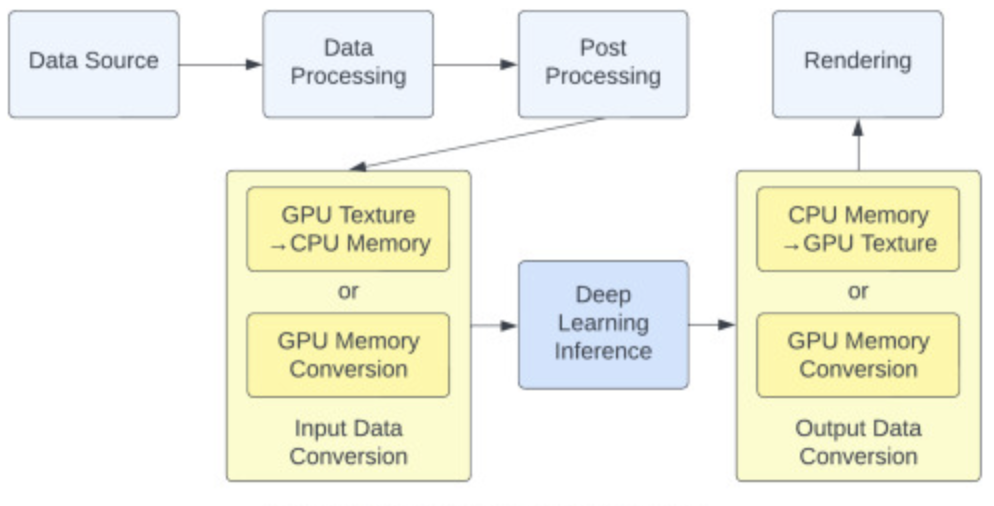
\includegraphics[width=1\linewidth]{images-pipeline/data.png}
                            \caption{Архитектура пайплайн с использованием сторонних фреймворков \hyperlink{[13]}{[13]}.}
                            \label{ris:netron}
                        \end{minipage}
                    \end{center}
                \end{figure}
                \item Недостаточная интеграция с визуальной логикой. Невозможность непосредственной передачи данных из шейдера в шейдер без выхода за пределы графического пайплайна затрудняет реализацию end-to-end решений.
            \end{enumerate}

            \subsection{Сравнение и анализ GPU-бэкендов}
            На данный момент поддержка GPU-инференса может быть реализована с использованием различных API:
            \begin{itemize}
                \item[-] Metal (только iOS/macOS): предоставляет унифицированный доступ к графическим и вычислительным функциям. Поддерживает низкоуровневый контроль, аналогичный OpenGL + OpenCL, но требует специфичной реализации под устройства Apple.
                \item[-] OpenGL ES: широко поддерживается на Android и используется в большинстве существующих приложений. Обеспечивает хорошую совместимость, но ограничен в вычислительных возможностях (отсутствие Compute Shader, ограниченные типы текстур и операций).
                \item[-] Vulkan: предлагает высокую производительность и низкие накладные расходы, но требует значительных усилий на реализацию и поддержку. Поддержка Vulkan-инференса ограничена на стороне фреймворков.
                \item[-] OpenCL: предоставляет более традиционную модель для вычислений на GPU, но плохо поддерживается на многих мобильных устройствах, особенно в бюджетном сегменте.
            \end{itemize}
            Исходя из широкой доступности, обратной совместимости и тесной интеграции с графикой, OpenGL ES остаётся наиболее приемлемым выбором для реализации описываемого пайплайна, особенно в задачах, связанных с обработкой видеопотока и визуализацией результатов непосредственно на экране устройства.
            
            \subsection{Обоснование выбора OpenGL в качестве платформы реализации}
            Учитывая вышесказанное, наиболее обоснованным является подход, при котором инференс нейросетевой модели реализуется напрямую на графическом конвейере средствами OpenGL. Такой подход позволяет:  использовать шейдеры как замену отдельным слоям модели (Conv2D, ReLU, BatchNorm и т.д.); хранить входы, выходы и веса в виде GPU-текстур без копирования на CPU; минимизировать количество операций ввода-вывода и переключений между контекстами; интегрировать обработку данных и визуализацию в едином render pass.
            
            Это решение открывает путь к реализации полноценных real-time приложений, использующих нейросети непосредственно в процессе отрисовки сцены, что особенно актуально для AR и компьютерного зрения на мобильных устройствах.

        \section{Выбор и описание модели для построения конвейера}
        Для реализации рассматриваемого real-time пайплайна на мобильных устройствах была выбрана модель Efficient Sub-Pixel Convolutional Network (ESPCN) \hyperlink{[10]}{[10]}. Данная модель зарекомендовала себя как эффективное решение для задач увеличения разрешения изображений, особенно в условиях ограниченного времени отклика, характерного для приложений дополненной реальности и компьютерного зрения на мобильных платформах.

        \begin{figure}[!h]
            \begin{center}
                \begin{minipage}[!h]{\linewidth}
                    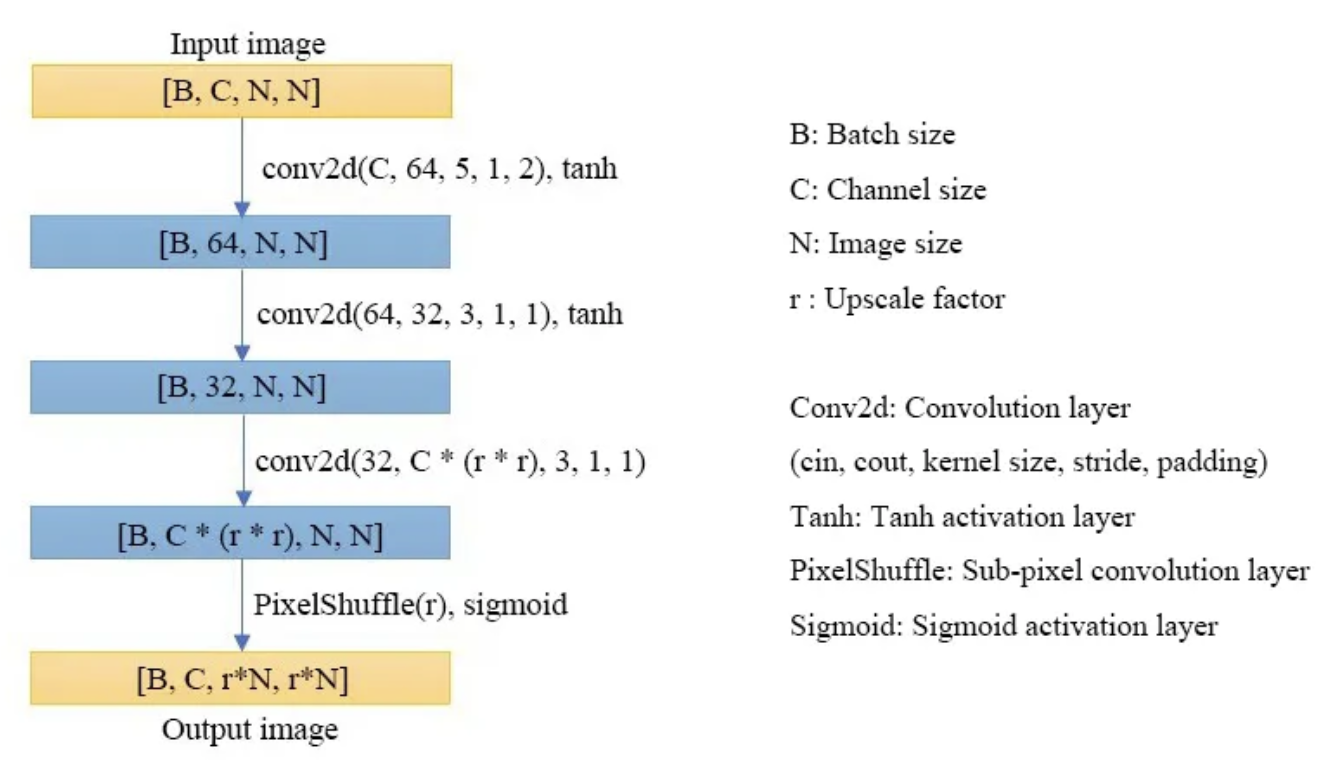
\includegraphics[width=1\linewidth]{images-pipeline/model.png}
                    \label{ris:netron}
                    \caption{Структура модели ESPCN \hyperlink{[10]}{[10]}}
                \end{minipage}
            \end{center}
        \end{figure}
        
        Модель ESPCN состоит из $L$ слоёв, где первые $L-1$ слоёв являются обычными сверточными слоями с активацией, а заключительный слой представляет собой субпиксельную перестановку — subpixel shuffle, обеспечивающую повышение пространственного разрешения выходного изображения. Основной идеей архитектуры является перенос вычислений, связанных с апсемплингом, в фазу свёртки с последующим дешевым и эффективным преобразованием тензора. Рассматриваемая конфигурация модели ESPCN включает следующие этапы:
        \begin{enumerate}
            \item Входной тензор: изображение в низком разрешении (Low-Resolution, LR) с формой $[B, C, N, N]$, где $B$ — размер батча, $C$ — число каналов, $N \times N$ — пространственное разрешение.
            \item Первый сверточный слой:
                \begin{itemize}
                    \item[-] Ядро размером $5 \times 5$, 64 фильтра;
                    \item[-] Активация: $\tanh(x)$ — используется вместо ReLU, так как модель ориентирована на восстановление цветовых текстур и деталей. Гладкая и ограниченная по выходу природа tanh помогает стабилизировать восстановление насыщенности в RGB-пространстве.
                \end{itemize}
            \item Второй сверточный слой:
                \begin{itemize}
                    \item[-] Ядро размером $3 \times 3$, 32 фильтра;
                    \item[-] Активация: $\tanh(x)$ — аналогично предыдущему слою, продолжает сжатие и уточнение признаков с учетом нелинейности.
                \end{itemize}
            \item Третий сверточный слой:
                \begin{itemize}
                    \item[-] Ядро размером $3 \times 3$, число выходных каналов: $C \times r^2$, где $r$ — коэффициент масштабирования;
                    \item[-] Без активации — это необходимо, чтобы не искажать значения, которые будут реорганизованы на следующем этапе.
                \end{itemize}
            \item Subpixel rearrangement (PixelShuffle):
                \begin{itemize}
                    \item[-] Выполняется перестановка элементов тензора с преобразованием формы с $[B, C \cdot r^2, N, N]$ в $[B, C, r \cdot N, r \cdot N]$;
                    \item[-] В отличие от методов интерполяции (bicubic, nearest), перестановка subpixel'ей не требует дополнительных вычислений на фазе апсемплинга, поскольку апсемплинг происходит структурно.
                \end{itemize}
            \item Финальная активация:
                \begin{itemize}
                    \item[-] Применяется $\sigma(x)$ (сигмоида), чтобы привести значения к диапазону $[0, 1]$, соответствующему нормированным значениям интенсивности пикселей.
                \end{itemize}
        \end{enumerate}

        \begin{figure}[!h]
            \begin{center}
                \begin{minipage}[!h]{0.39\linewidth}
                    \begin{center}
                        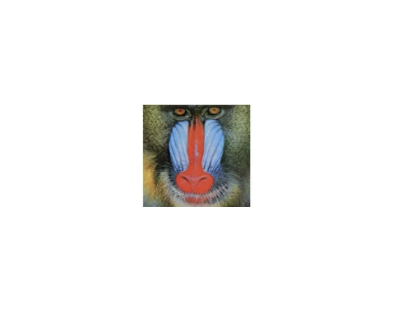
\includegraphics[width=1\linewidth]{images-pipeline/LR.png}
                        \label{ris:json}
                        \caption{Изображение в низком разрешении, передаваемое на вход модели \hyperlink{[10]}{[10]}}
                    \end{center}
                \end{minipage}
                \hfill
                \begin{minipage}[!h]{0.39\linewidth}
                    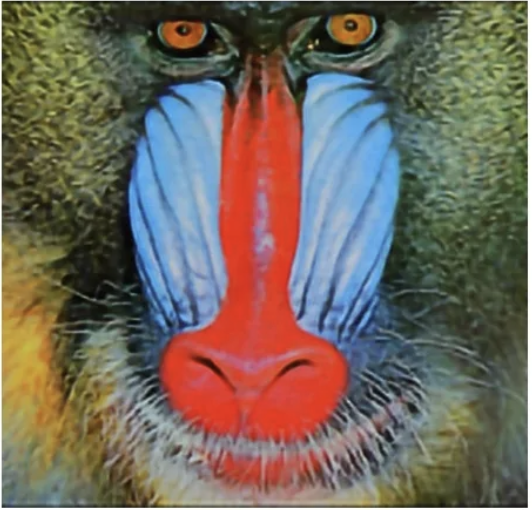
\includegraphics[width=1\linewidth]{images-pipeline/SR.png}
                    \label{ris:netron}
                    \caption{Результат обработки моделью ESPCN \hyperlink{[10]}{[10]}}
                \end{minipage}
            \end{center}
        \end{figure}

        \section{Применение задачи эффективного использования нейронных сетей на
графических процессорах}
        Эффективное использование нейронных сетей на графических процессорах (GPU) представляет собой одну из ключевых задач в современной вычислительной технике, особенно в условиях растущих требований к производительности и энергоэффективности в реальном времени. Данная задача находит широкое применение в различных отраслях, где требуется высокоскоростная обработка больших объёмов данных и выполнение сложных операций машинного обучения непосредственно на устройстве, без обращения к облачным вычислениям.

        В области дополненной и виртуальной реальности использование GPU для инференса нейросетей позволяет реализовывать интерактивные визуальные эффекты, отслеживание положения головы и рук, реконструкцию 3D-окружения и сегментацию объектов в кадре в реальном времени. Это особенно важно для мобильных и автономных AR-устройств, где ресурсы ограничены, а задержки должны быть минимальны. Примерами могут служить такие приложения, как виртуальные примерочные, геймплей с поддержкой жестового управления или медицинские симуляторы с адаптивным взаимодействием.
        
        В автомобильной промышленности нейросетевые модели, эффективно исполняемые на GPU, обеспечивают работу систем автономного вождения и помощи водителю: обнаружение объектов, распознавание дорожных знаков, оценка дорожной ситуации и предсказание поведения участников движения. Здесь критически важна не только точность моделей, но и способность обрабатывать потоки видеоданных в реальном времени на встраиваемых GPU, таких как NVIDIA DRIVE или другие специализированные SoC.
        
        Мобильная фотография и видеосъёмка также выигрывают от эффективного GPU-инференса. Такие задачи, как суперразрешение, шумоподавление, сегментация фона, коррекция освещения и применение нейросетевых фильтров, требуют высокопроизводительной обработки на устройстве. Использование GPU позволяет сократить время отклика интерфейса, снизить энергопотребление и увеличить качество выходного изображения.
        
        В индустрии безопасности и видеонаблюдения нейросетевые модели, выполняемые на GPU, применяются для распознавания лиц, аномалий, поведения и других задач видеоаналитики. Эффективность выполнения моделей на локальных графических процессорах позволяет реализовать интеллектуальные функции непосредственно на камерах или edge-устройствах, исключая необходимость передачи всего видеопотока в облако.
        
        Даже в сфере здравоохранения графические процессоры позволяют проводить инференс медицинских нейросетей непосредственно на диагностическом оборудовании — например, для классификации изображений МРТ или УЗИ в режиме реального времени. Это способствует ускорению постановки диагноза и снижению зависимости от удалённых серверов.
        
        Таким образом, эффективное использование нейронных сетей на графических процессорах является универсальной задачей, затрагивающей широкий спектр применений: от потребительских приложений и развлечений до промышленных, медицинских и транспортных систем. Улучшение алгоритмов выполнения, оптимизация памяти и параллелизма, а также архитектурные особенности современных GPU делают возможным расширение области применения нейросетей даже на энергоограниченных устройствах.
        
        В данной главе рассмотрена постановка задачи эффективного использования нейронных сетей на графических процессорах. Сделан обзор существующих реализаций и ключевых особенностей инференса на мобильных GPU. Выбрана модель для построения конвейера. Произведён обзор архитектуры модели. Приведены различные примеры применения данной задачи.
        
    \chapter{Разработка архитектуры пайплайна}
        Разрабатываемый пайплайн можно разделить на четыре основных этапа:
        \begin{enumerate}
            \item Преобразование модели в удобный для работы формат;
            \item Загрузка модели и манипуляции с ней;
            \item Генерация вычислительного графа и необходимая предобработка;
            \item Выполнение соответствующих операторов для обработки модели.
        \end{enumerate}
        
        \section{Преобразование модели}
            \begin{figure}[!h]
                \begin{center}
                    \begin{minipage}[!h]{0.38\linewidth}
                        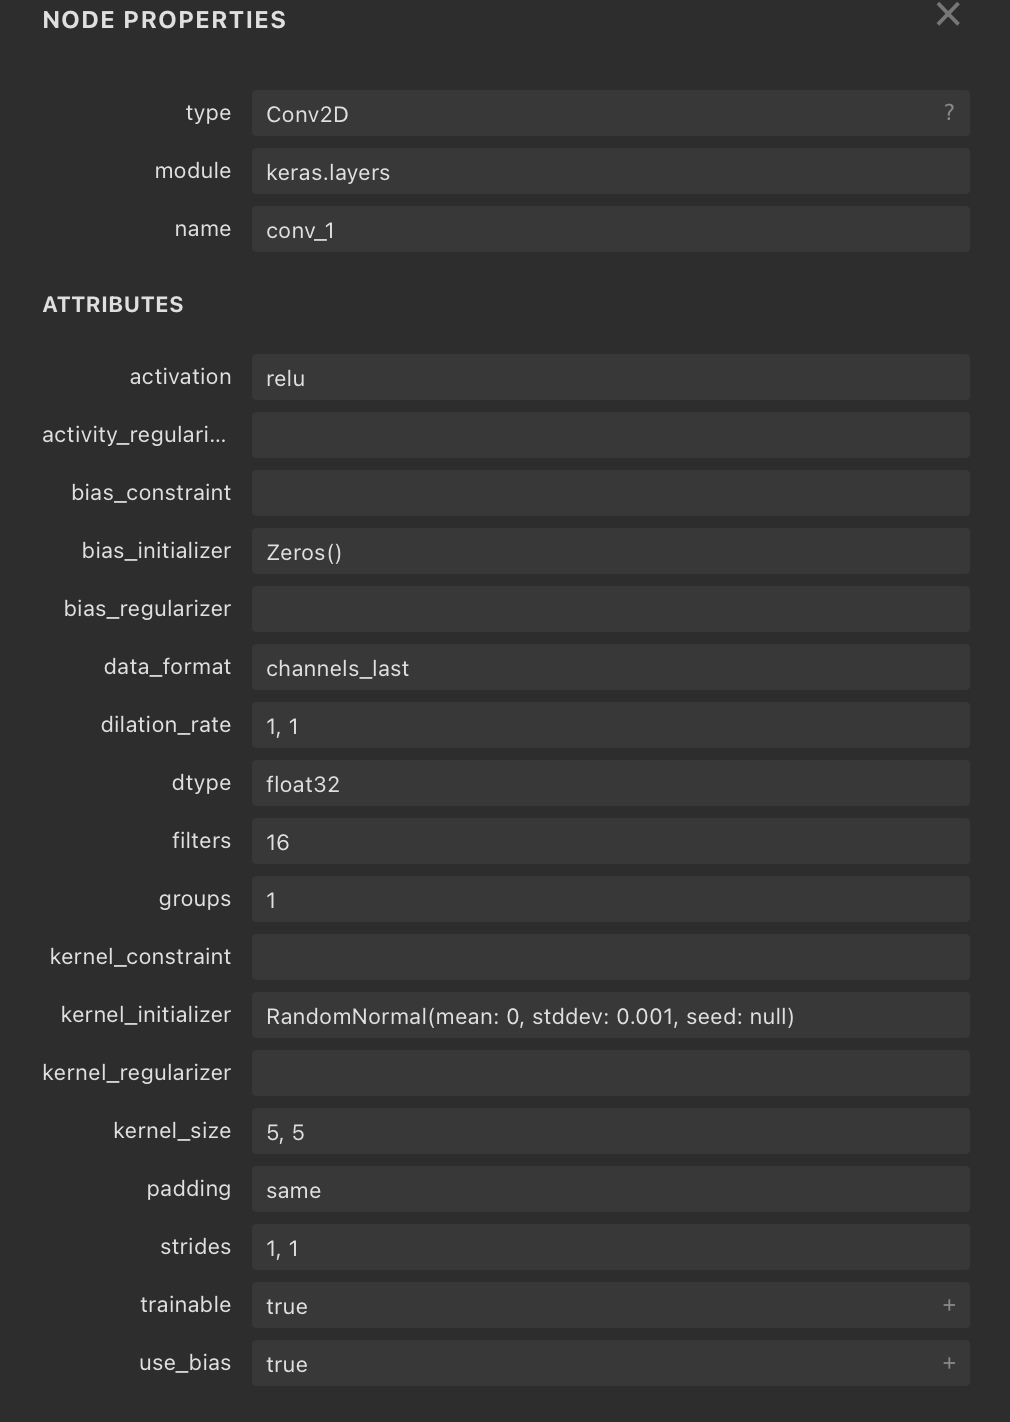
\includegraphics[width=1\linewidth]{images-pipeline/netron.png}
                        \label{ris:json}
                        \caption{Вид модели в веб-приложении Netron \hyperlink{[11]}{[11]}}
                    \end{minipage}
                    \hfill
                    \begin{minipage}[!h]{0.39\linewidth}
                        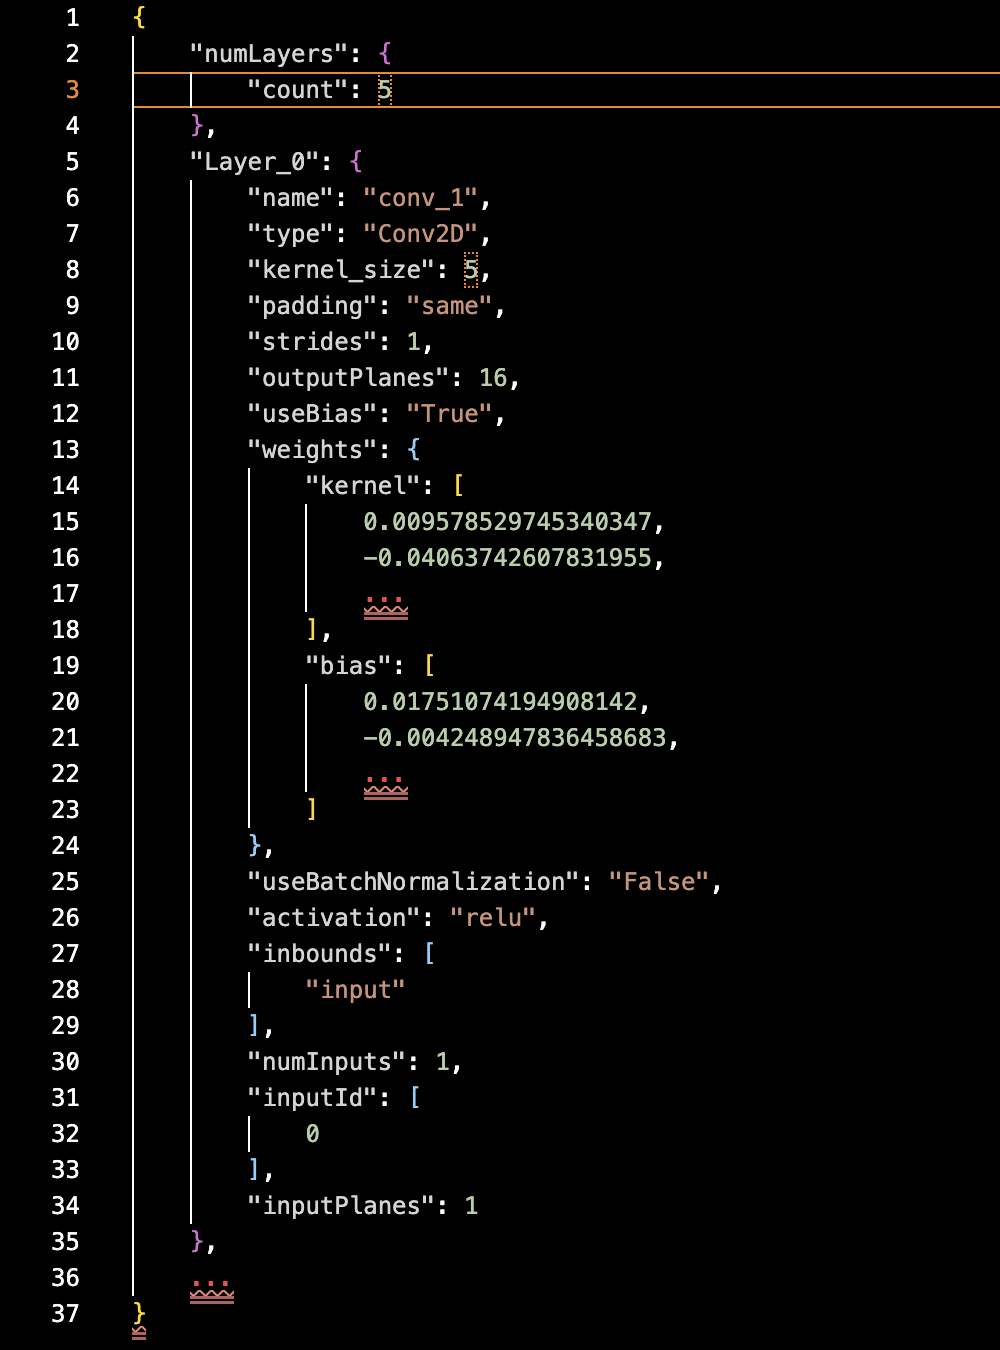
\includegraphics[width=1\linewidth]{images-pipeline/json.png}
                        \label{ris:netron}
                        \caption{Структура модели в созданном json файле} 
                    \end{minipage}
                \end{center}
            \end{figure}
            
            Так как большинство моделей обучается с помощью общедоступных фреймворков TensorFlow, Keras или PyTorch, они хранятся в соответствующих форматах. Следовательно, для их загрузки необходимо использовать один из перечисленных фреймворков, что является не совсем логичным в рамках разрабатываемого пайплайна из-за их размера. Поэтому для максимальной оптимизации и облегчения было принято решение о конвертации моделей в более удобный формат для загрузки — json файл. Для этого из модели необходимо извлечь всю необходимую информацию: количество слоев, тип слоя, входные параметры (ширина, высота, размер ядра), тип паддинга, веса текущего слоя, bias текущего слоя (дополнительная информация о природе данных для модели), какой тип активации использовать и т.д.

            Для этих целей был написан скрипт на языке Python, который на вход принимает модель в формате .h5 и возвращает json файл. Для его реализации используются сторонние библиотеки TensorFlow, для чтения входной модели, и json, для корректной работы со структурой файла и дальнейшей записи в соответствующий формат. Модель конвертируется один раз и далее пайплайн будет принимать только подготовленный формат (json файл). Также такой подход позволяет немного выиграть в памяти, требуемой для пайплайна. Во-первых, нет необходимости иметь стороннюю зависимость от TensorFlow, что отразилось бы на размере пайплайна. Во-вторых, json файл можно загрузить в память статически, что позволит избавиться от внешних зависимостей.
            
        \section{Загрузка модели и манипуляции с ней}
            Для загрузки модели были реализованы вспомогательные классы. Их основные функции заключаются в извлечении данных из json файла и хранении их в определённом формате в памяти. Класс ModelParser непосредственно отвечает за загрузку данных из файла и использует для этих целей доступный в открытом доступе фреймворк nlohmann::json. 

            При считывании графа из json файла применяется слияние слоев (эффективная оптимизация вычислительного графа). Данная техника позволяет значительно сократить количество слоев и, таким образом, снизить вычислительную стоимость инференса. Теоретически, если один из слоев представляет собой операцию element-wise или функцию map, он может быть объединён с предыдущим слоем. Например, слой activation можно объединить в один со слоем свертки или batch-нормализации, которые обычно за ним следуют.
            
            Также к такому методу можно прибегнуть и со слоем padding. Если его режим постоянный, повторяющийся или симметричный, то его можно объединить со следующим за ним. В следующем же слое объект OpenGL Sampler, прикреплённый к входной текстуре, обеспечит padding-функцию и тем самым уменьшит накладные расходы на проверку границ.

        \section{Архитектура фрагментного шейдера}
            В графическом пайплайне OpenGL фрагментный шейдер — это этап, который обрабатывает отдельные фрагменты для определения значения цвета соответствующих пикселей, присутствующих в данном фрагменте. Выходом фрагментного шейдера являются значения глубины и цвета, которые обычно записываются в render target или в framebuffer. Этап фрагментного шейдера работает совместно с этапом вершинного, который отвечает за предоставление координат интересующей квадратной области для последующей обработки её фрагментным шейдером.

            В отличие от вычислительных шейдеров, которые являются более гибкими и могут использоваться для более широкого круга задач, фрагментные шейдеры оптимизированы для рендеринга графики на экране (минус вычислительных шейдеров в том, что они менее универсальны, так как появились лишь в стандарте 4.6, который поддерживается не на всех устройствах). Этот тип рендеринга обычно предполагает параллельную обработку большого количества пикселей. По сравнению с вычислительными шейдерами, фрагментные продемонстрировали превосходство в производительности благодаря лучшей локальности данных и более эффективным схемам доступа к памяти. Например, в контекстно-зависимых алгоритмах, где каждое значение пикселя вычисляется и зависит от соседних значений, фрагментные работают с областью в пространстве экрана, что позволяет им использовать преимущества локальности данных и потенциально повысить производительность.
            
            Кроме того, фрагментные шейдеры обращаются к текстурным данным, которые хранятся в специальном типе памяти, называемом текстурным кэшем. Чаще всего это быстрее, чем обращение к данным, хранящимся в глобальной памяти, особенно если обращение к текстурным данным происходит неоднократно.
            
            В сверточных нейронных сетях (CNN) наиболее часто встречающейся операцией и, в свою очередь, одной из самых сложных, является свертка. Свертка в двух измерениях или на изображениях — это контекстно-зависимый алгоритм, в котором выходное значение вычисляется как сумма произведений ядра и сэмплированных входных пикселей. Это делает фрагментный шейдер подходящим вариантом использования при разработке механизма вывода для развертывания CNN.

            Исходя из вышеперечисленных плюсов фрагментного шейдера и особенностей архитектуры ESPCN (она является разновидностью архитектуры CNN), было принято решение в реализуемом пайплайне использовать именно их.

            При переводе операций, выполняемых CNN, в реализуемый пайплайн, входные данные слоя будут находиться в текстуре и обрабатываться вершинным и фрагментным шейдером. Затем данные записываются в render target. В зависимости от количества каналов на входе и выходе, данные могут храниться либо как текстура 2D, хранящая 4 канала, либо как массив текстур 2D, хранящий ещё 4 канала. Для операции свёртки в фрагментный шейдер веса будут передаваться через uniform buffer object или как входные uniform.
            
            Для универсальности, необходимые .glsl-файлы создаются непосредственно после извлечения данных из файла модели, при этом используются шаблоны (для каждого слоя они уникальны), написанные заранее. Для выбранной модели необходимо 3 шаблона: для слоя convolutional, activation и subpixel convolutional.
            
            Также стоит отметить, что каждый шейдер отвечает за генерацию 4-канального вывода в render pass. Для расчета слоя, имеющего более 4 выходов, требуется несколько .glsl-файлов и render pass, что и пришлось реализовывать для выбранной модели. Ниже приведена таблица, в которой перечислены слои и соответствующие им количества render pass:

            \begin{table}[H]
                \caption{\label{tab:canonsummary}Соотношение слоев модели ESPCN и количество render pass}
                \begin{center}
                    \begin{tabular}{|l|l|}
                        \hline
                        Модель ESPCN & Количество render pass \\
                        \hline
                        Layer 1: Conv2D output: $n \times n \times 16$ & Layer 1 output: 4 render passes \\
                        \hline
                        Layer 2: Conv2D output: $n \times n \times 16$ & Layer 2 output: 4 render passes \\
                        \hline
                        Layer 3: Conv2D output: $n \times n \times 4$ & Layer 3 output: 1 render pass \\
                        \hline
                        Layer 4: Subpixel output: $2n \times 2n \times 1$ & Layer 4 output: 1 render pass \\
                        \hline
                    \end{tabular}
                \end{center}
            \end{table}
        
        \subsection{Реализация свёрточного слоя Conv2D во фрагментном шейдере}
            В данном пункте описывается реализация архитектуры фрагментного шейдера для операции двумерной свёртки Conv2D. При разработке учитывалась производительность и поддержка различных конфигураций модели, так как они являются критически важными для удобной и эффективной интеграции в полноценный пайплайн.
    
            Реализация шейдера основана на использовании GLSL и API OpenGL ES, адаптированном для мобильных GPU (например, ARM Mali, Qualcomm Adreno). Данный шейдер поддерживает разнообразные конфигурации входных/выходных плоскостей, типов хранения весов, нормализации и схем паддинга. Архитектуру шейдера можно разделить на несколько уровней абстракции:
            \begin{enumerate}
                \item Через макрос FLOAT\_PRECISION задается требуемая точность вычислений mediump или highp, адаптируемая под целевое устройство. Обычно mediump используется для повышения производительности на мобильных устройствах. Highp, если требуется высокая числовая точность (например, при тонкой градации выходов). Выбор происходит в генеративной функции на C++ во время компиляции шейдера. Необходимая точность устанавливается вместо флага \_PLACEHOLDER\_PRECISION\_. В зависимости от параметра INPUT\_TEXTURE\_2D автоматически выбирается тип входных текстур: sampler2D или sampler2DArray;
                \lstinputlisting[language=c++, caption={Фрагмент шейдера с заданием точности вычислений}]{codeShaders/Conv2D/precision.glsl}
                
                \item Поддерживаются следующие методы паддинга:
                    \begin{itemize}
                        \item[-] CLAMPED\_PADDING. Стандартный паддинг реализованный в glsl, который задается при создании текстур в С++. Может использоваться GL\_NEAREST (возвращает значение элемента текстуры, которое находится ближе всего на расстоянии Манхэттена к центру пикселя) или же GL\_LINEAR (возвращает средневзвешенное значение четырех элементов текстуры, которые находятся ближе всего к центру  пикселя);
                        \item[-] CONST\_PADDING. Применяется нулевое или константное значение, которое задается как параметр на этапе компиляции шейдера;
                        \item[-] REPLICATE\_PADDING. В этом режиме используется отражение значения ближайшего корректного пикселя;
                        \item[-] CHECKBOARD\_PADDING. Применяет псевдослучайное отражение, создающее шахматный паттерн;
                        \item[-] REMOVE\_ZERO. Режим отсечения нулевых значений. Они заменяются на $0.001$.
                    \end{itemize}
                \lstinputlisting[language=c++, caption={Реализация методов replicatePadding и checkboardPadding}]{codeShaders/Conv2D/padding.glsl}
                Реализация паддинга выполняется в координатном пространстве нормализованных текстур. Методы replicatePadding и checkboardPadding обеспечивают генерацию корректных координат в условиях выхода за границы текстуры;
                
                \item Реализованы три режима работы с весами:
                    \begin{itemize}
                        \item[-] USE\_WEIGHT\_CONSTANTS. Все веса встроены в код. Они передаются как константы на этапе компиляции шейдера. Для этого используются специальные флаги \_PLACEHOLDER\_WEIGHT1\_VEC\_CONSTANTS\_. Когда веса извлечены из json файла модели, они записываются в шейдер на место данных указателей. Такой подход позволяет использовать один шаблон для нескольких render pass, что является более универсальным подходом, чем создание отдельных шейдеров на каждый render pass. Также стоит отметить, что данный режим оптимален для render pass с небольшим количеством использованных весов. Этот режим является наиболее эффективным по скорости выполнения, так как в нем отсутствуют расходы на обращение к памяти текстуры или SSBO;
                        \lstinputlisting[language=c++, caption={Фрагмент шейдера с константным заданием весов}]{codeShaders/Conv2D/constWeights.glsl}
                        \item[-] USE\_WEIGHT\_TEXTURES. В данном режиме веса загружаются как текстуры во время выполнения шейдера. Данный режим оптимален для render pass с большим количеством используемых весов, но работает немного дольше чем USE\_WEIGHT\_CONSTANTS, так как необходимо каждый раз обращаться к памяти текстуры;
                        \lstinputlisting[language=c++, caption={Фрагмент шейдера с заданием весов через текстуры}]{codeShaders/Conv2D/textureWeights.glsl}
                        \item[-] USE\_WEIGHT\_BUFFERS. В этом режиме веса передаются как SSBO (shader storage buffer object — это буферный объект, который используется для хранения и извлечения данных на языке glsl). Данный режим позволяет использовать значительно большие веса, по сравнению с USE\_WEIGHT\_TEXTURES. Спецификация OpenGL гарантирует, что размер UBO (uniform buffer object — объект позволяющий получить текстуру, передаваемую из С++, на стороне glsl и манипулировать ей) может быть до 16 КБ. В свою очередь, SSBO могут быть размером до 128 МБ, но большинство реализаций позволят выделить размер до предела памяти графического процессора. С другой стороны, чтение данных из SSBO, при прочих равных условиях, скорее всего, будет медленнее, чем доступ к UBO. SSBO, как правило, доступны как буферные текстуры, в то время как доступ к данным UBO осуществляется через чтение внутренней памяти, доступной шейдером. Поэтому данный режим используется для render pass с самым тяжелым набором весов, но приводит к незначительной потере в скорости отработки.
                        \lstinputlisting[language=c++, caption={Фрагмент шейдера с заданием весов через SSBO}]{codeShaders/Conv2D/ssboWeights.glsl}
                    \end{itemize}
                Каждый компонент (RGBA) выходного пикселя может обрабатываться через отдельную плоскость весов. Всего предусмотрено до 16 наборов весов (weights1–weights16), что позволяет покрыть до четырех выходных каналов по 4 компонента каждый. Для этого на этапе компиляции шейдера задаются необходимые макросы формата USE\_COMPONENT\_\{R, G, B, A\}\_\ PLANE\_\{0-3\};
                
                \item Шейдер поддерживает операцию батч нормализации. В случае активации USE\_BATCH\_NORMALIZATION шейдер ожидает на вход параметры gamma, beta, movingMean, movingVariance. Эти параметры применяются к выходу после свёртки, в соответствии с уравнением:
                \begin{equation}
                \hat{x} = \gamma \cdot \frac{x - \mu}{\sqrt{\sigma^2 + \epsilon}} + \beta
                \end{equation}
                Данные параметры могут либо передаваться как UBO во время выполнения шейдера, либо передаваться как константы на этапе компиляции шейдера. Во втором случае используются специальные флаги формата \_PLACEHOLDER\_\{BETA, GAMMA, MOVINGMEAN, MOVINGVARIANCE\}\_. Когда веса извлечены из json файла модели, они записываются в шейдер на место данных указателей. Такой подход позволяет использовать один шаблон для нескольких render pass, что является более универсальным подходом, чем создание отдельных шейдеров на каждый render pass;
                \lstinputlisting[language=c++, caption={Фрагмент шейдера с заданием параметров для батч нормализации}]{codeShaders/Conv2D/batch.glsl}
                
                \item Вывод результатов осуществляется в выходные плоскости o\_pixel, o\_pixel1 и т.д., каждая из которых соответствует вектору vec4. Их количество задается через соответствующие макросы. Это позволяет эффективно параллелить свёртки с множеством выходных каналов.
                \lstinputlisting[language=c++, caption={Фрагмент шейдера с заданием выходных плоскостей}]{codeShaders/output.glsl}
            \end{enumerate}
            
            Основная функциональность слоя Conv2D реализована в функции main(). Данная функция управляет основным циклом обработки входных данных, обеспечивая параллельное выполнение операций над пикселями.
    
            В начале функции происходит преобразование координат фрагмента gl\_FragCoord в координаты базового пикселя с учетом параметра NUM\_STRIDE, определяющего шаг свертки. Данный параметр задается во время компиляции шейдера. Он позволяет применять свертку с пропусками strided convolution, аналогично тому, как это делается в сверточных нейронных сетях.
            
            Далее функция вычисляет координаты выборки текстурных значений texCoords и координаты весов свертки weightsCoords для всего окна ядра свертки размером $NUM\_KERNEL\_SIZE \times NUM\_KERNEL\_SIZE$. Это обеспечивает модульность, позволяя работать с типами паддинга, перечисленными выше, и корректно обрабатывать граничные условия.
            
            Сама операция свертки реализована как вложенный цикл по размерам ядра. Для каждой группы из четырёх входных каналов (вектор vec4) происходит выборка значений из текстур и их свертка с весами. После суммирования значений свертки для каждого канала s, s1, s2, s3, к результатам добавляется соответствующее значение смещения bias. Далее, если включена батч нормализация USE\_BATCH\_NORMALIZATION, каждый выходной канал нормализуется с использованием заранее вычисленных параметров среднего значения movingMean, дисперсии movingVariance, а также масштабирующих коэффициентов gamma и смещений beta.
    
            Далее применяется функция активации, которая задается через генеративную функцию из С++, которая работает на этапе компиляции шейдера. Активация устанавливается после применения батч нормализации, если та включена. Это позволяет использовать одну и ту же структуру шейдера для различных архитектур нейронных сетей. Ниже приведены примеры реализованных функций активации:
            \begin{itemize}
                \item[-] \textbf{ReLU:} s = max(s, vec4(0.0));
                \item[-] \textbf{ReLU6:} s = clamp(s, vec4(0.0), vec4(6.0));
                \item[-] \textbf{Tanh:} s = tanh(s);
                \item[-] \textbf{Sigmoid:} s = vec4(1.0f) / (vec4(1.0f) + exp(-s));
                \item[-] \textbf{LeakyReLU (с параметром alpha):} s = max(s, (s * vec4(alpha)));
                \item[-] \textbf{SiLU (Swish):} s = s * vec4(1.0f) / (vec4(1.0f) + exp(-s));
            \end{itemize}
            
            После применения активации, данные записываются обратно в выходные буферы. Этот подход обеспечивает параллельную запись нескольких выходных плоскостей, при необходимости — для ускорения инференса при работе с несколькими каналами.
            \lstinputlisting[language=c++, caption={Фрагмент шейдера с записью результата в  выходные плоскости}]{codeShaders/output.glsl}
            
            Таким образом, данный шейдер реализует обобщённую версию слоя свёртки с возможностью использования различных оптимизаций и параметров. Это позволяет легко адаптировать её к различным архитектурам нейросетей, сохраняя при этом эффективность вычислений на GPU.
        
        \subsection{Реализация слоя активации Activation во фрагментном шейдере}
            Слои активации являются неотъемлемой частью нейросетевых архитектур, обеспечивая необходимую нелинейность в процессе вычислений. Их реализация в GPU-конвейере требует балансировки между производительностью и точностью, особенно в условиях ограниченных ресурсов мобильных графических процессоров (например, ARM Mali, Qualcomm Adreno).
            
            В данном пункте непосредственно описывается архитектура и особенности реализации слоя активации с использованием фрагментного шейдера в рамках конвейера инференса на GPU. В реализации используется фрагментный шейдер на языке GLSL с интерфейсом OpenGL ES. Он адаптирован под текстурные представления тензоров в формате 2D или 2DArray.
            
            Фрагментный шейдер предназначен для применения функции активации к тензору признаков, представленному в виде текстурных срезов. Универсальность шейдера достигается за счёт использования макросов, позволяющих адаптировать код под различное количество выходных плоскостей, задаваемое параметром PLANE\_COUNT, и типа входных текстур, которые могут быть либо в формате 2D, либо в формате 2DArray. Также в данном шейдере реализовано использование различных функций активации с помощью флага \_PLACEHOLDER\_ACTIVATION\_. Данные функции выбираются на этапе компиляции шейдера и передаются напрямую из кода C++.
            
            Для обеспечения совместимости с разными точками использования шейдера в графическом конвейере, в начале файла определена точность вычислений:
            \lstinputlisting[language=c++, caption={Фрагмент шейдера с заданием точности вычислений}]{codeShaders/Activation/precision.glsl}
            Параметр FLOAT\_PRECISION позволяет выбрать требуемую точность вычислений — обычно это или mediump для повышения производительности на мобильных устройствах, или highp, если требуется высокая числовая точность (например, при тонкой градации выходов). Выбор происходит в генеративной функции на C++ во время компиляции шейдера. Необходимая точность устанавливается вместо флага \_PLACEHOLDER\_PRECISION\_.
            
            Выходные переменные шейдера задаются в формате:
            \lstinputlisting[language=c++, caption={Фрагмент шейдера с заданием выходных плоскостей}]{codeShaders/outputBind.glsl}
            Такой подход позволяет записывать данные в несколько render target (Multiple Render Targets, MRT), что актуально при обработке нескольких каналов одновременно. Для вычисления нейросетевых слоев это особенно актуально, так как обычно слои содержат довольно много информации и, следовательно, шейдер, для большей эффективности, должен обрабатывать её параллельно.
            
            Внутри функции main() производится определение выходной координаты текущего фрагмента, а для текстур формата 2DArray дополнительно выбирается слой. Это позволяет обеспечить выбор конкретного среза входного тензора при обработке batched-инференса или channel-major представлений.
            \lstinputlisting[language=c++, caption={Фрагмент шейдера с определением слоя и входных координат}]{codeShaders/Activation/coord.glsl}
            
            Считывание данных из входной текстуры осуществляется функцией texelFetch. Шейдер реализует гибкую систему выбора между 2D и 2DArray текстурами на основе установленного макроса. Аналогично инициализируются переменные для других слоёв, если $PLANE\_COUNT > 1$. Такая структура позволяет одновременно обрабатывать до четырёх каналов, загружая данные из разных слоёв массива текстуры.
            \lstinputlisting[language=c++, caption={Фрагмент шейдера со считыванием данных из входной текстуры}]{codeShaders/Activation/fetch.glsl}
            
            Ключевым элементом шейдера является применение функции активации, задаваемой флагом \_PLACEHOLDER\_ACTIVATION\_. Это позволяет использовать одну и ту же структуру шейдера для различных типов активаций. Ниже приведены примеры реализованных функций активации:
            \begin{itemize}
                \item[-] \textbf{ReLU:} s = max(s, vec4(0.0));
                \item[-] \textbf{ReLU6:} s = clamp(s, vec4(0.0), vec4(6.0));
                \item[-] \textbf{Tanh:} s = tanh(s);
                \item[-] \textbf{Sigmoid:} s = vec4(1.0f) / (vec4(1.0f) + exp(-s));
                \item[-] \textbf{LeakyReLU (с параметром alpha):} s = max(s, (s * vec4(alpha)));
                \item[-] \textbf{SiLU (Swish):} s = s * vec4(1.0f) / (vec4(1.0f) + exp(-s));
            \end{itemize}
            
            Эти функции выбираются на этапе генерации GLSL-кода из C++ и вставляются как инлайновые фрагменты в шейдер. Это позволяет обеспечить высокую гибкость в использовании данного шейдера для нейронных сетей с различной архитектурой. Также такой подход минимизирует накладные расходы на условные операторы и обеспечивает максимально возможную производительность.
            
            После применения активации, данные записываются обратно в выходные буферы. Этот подход обеспечивает параллельную запись нескольких выходных плоскостей. Использование MRT позволяет снизить количество проходов по тензору и улучшить общую пропускную способность GPU.
            \lstinputlisting[language=c++, caption={Фрагмент шейдера с записью результата в  выходные плоскости}]{codeShaders/output.glsl}
            
            Таким образом, полученный фрагментный шейдер представляет собой универсальный и модульный способ реализации слоя активации. Гибкость, достигаемая за счёт флагов и макросов, делает его легко адаптируемым под различные архитектуры нейросетей и типы функций активации. Возможность поддержки MRT (Multiple Render Targets) и выбор между текстурами формата 2D или 2DArray позволяет интегрировать его в сложные вычислительные графы с минимальными издержками по производительности.
        
        \subsection{Реализация слоя Subpixel во фрагментном шейдере}
            В данном пункте рассматривается реализация слоя Subpixel с учётом производительности и особенностей исполнения на графическом процессоре мобильного устройства. В реализации используется фрагментный шейдер на языке GLSL с интерфейсом OpenGL ES.
            
            Слой subpixel merge применяется в случае, когда выход предыдущего слоя представлен в субпиксельной (channel-wise) форме. Это характерно для моделей с апсемплингом по принципу pixel shuffle (sub-pixel convolution) или при агрегации данных из различных пространственных компонент. В результате работы таких слоев данные пространственно интерполируются в каналах, и задача слоя subpixel merge состоит в том, чтобы корректно восстановить из них полное изображение.
    
            Приведённый шейдер реализует преобразование из субпиксельного представления в обычное 2D изображение. Входной тензор представлен в виде 2DArray — набор 2D текстур, разбитых по слоям (channel groups).
            
            Параметр FLOAT\_PRECISION позволяет выбрать требуемую точность вычислений — обычно это или mediump для повышения производительности на мобильных устройствах, или highp, если требуется высокая числовая точность (например, при тонкой градации выходов). Выбор происходит в генеративной функции на C++ во время компиляции шейдера. Необходимая точность устанавливается вместо флага \_PLACEHOLDER\_PRECISION\_.
            \lstinputlisting[language=c++, caption={Фрагмент шейдера с заданием точности вычислений}]{codeShaders/Subpixel/precision.glsl}
            
            Операция объединения основана на реконструкции субпиксельной информации в соответствии с её исходной позицией.
    
            Сначала шейдер корректирует координаты пикселя, так как в OpenGL по умолчанию используется центр пикселя $x + 0.5,\ y + 0.5$. Для согласованности с индексами модели используется сдвиг координат: $gl\_FragCoord.x\ -\ 0.5$ и $gl\_FragCoord.y\ -\ 0.5$.
            
            Далее вычисляется индекс текущей компоненты. Такой подход соответствует порядку развёртки, при котором сабпиксели укладываются в строку или блоки.
            \lstinputlisting[language=c++, caption={Фрагмент шейдера с вычислением индекса текущей компоненты}]{codeShaders/Subpixel/index.glsl}
            
            В случае, если $kernelSize\ \ge\ 4$, вводится поддержка многослойного inputTextures. В таком варианте каждый слой представляет группу из 4 каналов (является форматом vec4).
            
            Непосредственно для чтения значений субпикселей используется функция texelFetch, так как необходим доступ к точным координатам без интерполяции. Координаты вычисляются по формуле:
            \begin{equation}
            uvt = \left( \left\lfloor \frac{x}{kernelSize} \right\rfloor,\ \left\lfloor \frac{y}{kernelSize} \right\rfloor,\ \text{layer} \right)
            \end{equation}
            Функция texelFetch позволяет прочитать конкретный texel из текстуры. Одним из важных параметров в функции является последний, он указывает уровень детализации в текстуре, из которой будет извлечен texel. Стоит отметить, что в комбинации с таким расчетом координат она позволяет найти texel, соответствующий группе нужных для расчета субпикселей.
            \lstinputlisting[language=c++, caption={Фрагмент шейдера с расчетом координат и применением функции texelFetch}]{codeShaders/Subpixel/fetch.glsl}
            
            Далее, в зависимости от значения посчитанной компоненты, выбирается необходимый канал выбранного texel.
            \lstinputlisting[language=c++, caption={Фрагмент шейдера с выбором}]{codeShaders/Subpixel/comp.glsl}
            
            В зависимости от установленных макросов, выход может быть представлен в различных форматах. Реализованы три варианта:
            \begin{itemize}
                \item[-] OUTPUT\_Y2RG. В данном режиме выходным форматом будет являться vec2. Это используется, например, для кодирования знаковых величин в два канала Red и Green;
                \item[-] OUTPUT\_Y2RG\_HALF. В этом режиме значение делится пополам по модулю и присваивается либо первому, либо второму каналу:
                \begin{equation}
                \mathbf{o\_pixel} =
                \begin{cases}
                \begin{pmatrix}
                0 \\
                -\dfrac{s}{2}
                \end{pmatrix}, & \text{если } s < 0 \\
                \\
                \begin{pmatrix}
                \dfrac{s}{2} \\
                0
                \end{pmatrix}, & \text{если } s \geq 0
                \end{cases}
                \end{equation}
                Это эффективно для хранения в формате unsigned outpu;
                \item[-] Без OUTPUT\_Y2RG. В таком режиме, выход будет предствалять собой скалярное значение float, напрямую представляющее прочитанный субпиксель.
            \end{itemize}
            
            Такая конфигурация необходима при последовательной постобработке в других частях модели или при ограничениях на выходной формат текстурного буфера.
    
            Стоит отметить, что была произведена некоторая оптимизация реализованного шейдера для предотвращения возможных потерь. Для этого были реализованы следующие пункты:
            \begin{itemize}
                \item[-] Отказ от операций ветвления на высоких уровнях. Хотя if (component == ...) присутствует, количество ветвлений ограничено и выполняется в пределах одного warp;
                \item[-] Использованы целочисленные индексы и функция texelFetch. Таким образом были минимизированы неопределенности, связанные с линейной интерполяцией и ошибками округления;
                \item[-] На вход шейдер принимает формат 2DArray, что позволяет экономично упаковавать входные каналы. Это важно при ограничении числа текстурных юнитов, которые могут быть задействованы;
                \item[-] Задействована масштабируемость по kernelSize. Такая архитектура позволяет масштабировать число субпикселей, просто увеличивая kernelSize и глубину inputTextures.
            \end{itemize}
            
            Таким образом, реализованный слой subpixel merge является высокоэффективным способом пространственной реконструкции данных, представленных в субпиксельной форме. Его структура позволяет эффективно использовать GPU на мобильных устройствах, избегая избыточных вычислений и обеспечивая точный контроль над размещением данных. Гибкость реализации, задаваемая через макросы, позволяет использовать данный шейдер с различными архитектурами нейронных сетей без дополнительных доработок.
        
        \section{Реализация и архитектура вершинного шейдера}
            Для корректной работы любого фрагментного шейдера в графическом пайплайне необходимо определить соответствующий вершинный шейдер, который обеспечит правильную трансформацию входных данных и передачу необходимых атрибутов (например, координат текстурирования) на фрагментный этап. В разработанном пайплайне для мобильных устройств была принята стратегия использования единого универсального вершинного шейдера для всех слоёв модели, реализуемых на графическом процессоре GPU. Такой подход позволяет упростить управление графическим конвейером, уменьшить количество переключений программ и, следовательно, улучшить производительность в условиях ограниченных вычислительных ресурсов мобильных устройств.
    
            На этапе проектирования был выбран метод отрисовки полноэкранного треугольника вместо стандартной квадратной геометрии (из двух треугольников), покрывающей всё изображение. Это решение снижает накладные расходы на вершинную обработку, поскольку требуется обработка всего трёх вершин, а не шести, как в случае с двумя треугольниками. При этом достигается полное покрытие области рендеринга без визуальных артефактов благодаря особенностям растеризации в OpenGL ES.
            
            Ниже приведён код вершинного шейдера, реализующего описанную стратегию:
            \lstinputlisting[language=c++, caption={Шаблон вершинного шейдера для слоя activation}]{codeShaders/vertex.glsl}

            Шейдер использует встроенный индекс gl\_VertexID для выбора одной из трёх заранее определённых вершин. Каждая вершина задаётся как четырёхкомпонентный вектор vec4(x, y, z, w), где:
            \begin{itemize}
                \item[-] x, y — координаты вершины в нормализованном пространстве экрана (NDC);
                \item[-] z, w — соответствующие UV-координаты, передаваемые во фрагментный шейдер через переменную v\_uv.
            \end{itemize}
            
            Выбор значений координат произведён с учётом поведения растеризатора, чтобы треугольник, заданный следующими вершинами:
            \begin{enumerate}
                \item (-1, -1) — нижний левый угол экрана, UV = (1, 1);
                \item (3, -1) — точка за пределами правого нижнего угла, UV = (1, -1);
                \item (-1, 3) — точка за верхним левым краем, UV = (-1, 1);
            \end{enumerate}
            покрывал всю прямоугольную область экрана без пробелов. Данный метод называется Fullscreen Triangle Rendering и является устоявшейся практикой для rendering в реальном времени, поскольку устраняет потенциальные швы между двумя треугольниками, минимизирует количество обрабатываемых вершин в несколько раз и улучшает кэширование и эффективность GPU во время рендеринга.

            Особенность передачи UV координат заключается в использовании нестандартного диапазона: от -1 до 1, в отличие от традиционного диапазона [0, 1]. Это обосновано тем, что в большинстве слоёв нейросетевого инференса (например, activation, elementwise, conv2D и т.д.) обрабатываются не визуальные текстуры, а тензорные данные, интерпретируемые как текстуры с плавающей точкой. Диапазон координат может быть перекалиброван во фрагментном шейдере для прямого индексирования в текстуру (например, через нормализацию координат в зависимости от размера тензора). Это позволяет добиться высокой универсальности кода и облегчить масштабирование архитектуры под различные разрешения входных данных.
            
            Также реализация общего вершинного шейдера оправдана тем, что большинство операций инференса в графическом конвейере фокусируются на покрытии всего пространства тензора (или его проекции в виде текстуры). Сюда относятся:
            \begin{itemize}
                \item[-] нелинейные активации (ReLU, Sigmoid);
                \item[-] нормализация;
                \item[-] элементные операции (Add, Multiply);
                \item[-] свёртки с малым ядром и шагом 1.
            \end{itemize}
            
            Во всех этих случаях отсутствует необходимость в индивидуальной геометрии, так как входные и выходные данные представлены текстурами одинакового размера. Таким образом, полноэкранный треугольник идеально подходит в качестве геометрической основы.

            Таким образом, представленный вершинный шейдер является ключевым элементом унифицированного рендер-пайплайна для инференса нейронных сетей на мобильных устройствах в условиях реального времени. Использование полноэкранного треугольника позволяет достичь высокой производительности и минимизации накладных расходов, а стратегия разделения координат (позиция + UV) обеспечивает достаточную гибкость при адресации тензорных данных. В дальнейшем данный шейдер может быть легко расширен, например, для поддержки различного масштабирования, кропа или батчей в рамках одного вызова рендеринга.

        \section{Архитектура и реализация ядра инференса}
            Для обеспечения максимально эффективной работы модели нейронной сети в рамках конвейера OpenGL был разработан специализированный исполнительный механизм — Inference Core, реализующий архитектурную обвязку над моделью в виде графа операций. Эта архитектура позволяет трактовать каждый фрагмент вычислений как единицу рендеринга, обеспечивая непосредственную интеграцию с текстурами GPU и минимизацию накладных расходов на копирование данных между CPU и GPU.

            После предварительной загрузки и разбора нейросетевой модели она трансформируется во внутреннее представление — InferenceGraph, который содержит вершины (узлы), соответствующие операциям модели, и ребра, определяющие поток данных. Каждая вершина в этом графе сопоставляется с отдельным вычислительным этапом (RenderStage), который, в свою очередь, может состоять из одного или нескольких render pass. Это позволяет гибко разделять сложные операции на подэтапы с возможностью детального контроля рендеринга.
            
            \begin{algorithm}[H]
            \caption{Инициализация ядра инференса}
            \label{alg:init}
            \begin{algorithmic}[1]
            \Function{init}{}
                \State $m\_Layers \gets \text{InferenceGraph.Layers}$
                \For{$i \gets 0$ \textbf{to} $layers.\text{size()} - 1$}
                    \State $m\_Stage[i] \gets \text{new RenderStage()}$
                    \State $m\_Stage[i].Layer \gets m\_Layers[i]$
                    \For{$j \gets 0$ \textbf{to} $m\_Layers[i].\text{Inputs.size()} - 1$}
                        \State $input \gets m\_Layers[i].Inputs[j]$
                        \If{$input.\text{IsStageOutput}$}
                            \State $texture \gets input.\text{m\_StageOutputs}[0].\text{Texture}$
                        \Else
                            \State $texture \gets ModelInputs[j].\text{Texture}$
                        \EndIf
                        \State $stage[i].\text{m\_StageInputs}[j].\text{Texture.Attach}(Texture)$
                    \EndFor
                    \State $stage[i].\text{m\_StageOutputs}[0].\text{Texture.Allocate}()$
                    \For{$k \gets 0$ \textbf{to} $m\_Layers[i].\text{Passes.size()} - 1$}
                        \State $stage[i].\text{RenderPasses}[k].\text{Init}()$
                    \EndFor
                \EndFor
            \EndFunction
            \end{algorithmic}
            \end{algorithm}

            Инициализация пайплайна осуществляется через функцию init(), задача которой — развернуть и связать между собой все этапы рендеринга согласно структуре InferenceGraph. На этом этапе происходит:
            \begin{enumerate}
                \item Создание объектов RenderStage для каждой вершины графа;
                \item Идентификация входных и выходных связей между вершинами;
                \item Привязка текстур выходов/входов с учетом возможных переиспользований;
                \item Выделение GPU-ресурсов (через вызов .allocate()) для выходных текстур;
                \item Инициализация всех render passes внутри каждого RenderStage.
            \end{enumerate}
            Это дает возможность избежать повторного выделения памяти на каждом кадре и обеспечивает возможность потоковой передачи данных между узлами через OpenGL текстуры.

            Функция run() запускает инференс в два этапа: сначала происходит привязка входных текстур к соответствующим входам модели, затем производится последовательный запуск всех render pass каждого RenderStage. Такой подход позволяет эффективно реализовать потоковую передачу данных и избежать синхронизаций с CPU.
            \begin{algorithm}[H]
            \caption{Функция выполнения инференса}
            \label{alg:run}
            \begin{algorithmic}[1]
                \Function{run}{}
                    \For{$i \gets 0$ \textbf{to} $length(m_InputTextures)$}
                        \State $m\_ModelInputs[i].Texture(0).Attach(m\_InputTextures[i])$
                    \EndFor
                    \For{$j \gets 0$ \textbf{to} $m\_RenderStages.size()$}
                        \State $renderPasses \gets m\_RenderStages[j].RenderPasses$
                        \For{$k \gets 0$ \textbf{to} $renderPasses.size()$}
                            \State $renderPasses[k].Run()$
                        \EndFor
                    \EndFor
                \EndFunction
            \end{algorithmic}
            \end{algorithm}

            Предложенная реализация обладает рядом преимуществ, важных для разработки мобильного пайпалана, таких как:
            \begin{itemize}
                \item[-] Унификация входных и выходных данных в виде OpenGL текстур позволяет устранять избыточные копирования и повысить производительность;
                \item[-] Динамическая регистрация операторов без необходимости переписывать центральную часть пайплайна;
                \item[-] Лёгкость расширения, что особенно важно для задач, требующих кастомных слоёв (например, для обработки глубины, сегментации или flow);
                \item[-] Малые накладные расходы, т.к. вычисления организованы с учётом locality и переиспользования GPU ресурсов.
            \end{itemize}

            В данной главе рассмотрена архитектура и реализация пайплайна для эффективного использования нейронных сетей на графических процессорах. Сделан обзор реализованного преобразования модели из формата .h5 в json файл. Описан алгоритм загрузки модели и манипуляций, произведённых с ней, для ускорения работы пайплайна. Рассмотрена архитектура и реализация фрагментных шейдеров для слоёв Conv2D, Activation и Subpixel. Также описана архитектура и реализация вершинного шейдера и ядра инференса.

    \chapter{Тестирование пайплайна и сравнение с существующими фреймворками}
        Для формализации эффективности использования нейросетей на GPU и описания критериев тестирования построенного пайплайна введем следующие показатели:
        \begin{enumerate}
            \item Latency (задержка) — среднее время выполнения одного инференса после стадии прогрева, включая только вычислительные затраты внутри графического конвейера;
            \item Data Transfer Overhead (временные издержки на передачу данных) — суммарное время, затрачиваемое на передачу входных и выходных тензоров между GPU и CPU, вне рамок непосредственного инференса;
            \item Pipeline Initialization Cost (затраты на инициализацию пайплайна) — время, необходимое для компиляции шейдеров, создания буферов и настройки всех этапов вычислительного графа перед началом обработки.
        \end{enumerate}

        Для сравнения эффективности реализованного пайплайна выбраны фреймворк MediaPipe и TFLite с делегатом GPU, так как они являются наиболее распространёнными и популярными в рамках рассматриваемой задачи. Все три реализации будут использовать одинаковую среду: входное видео, телефон/ноутбук, нейросеть ESPCN.

        \section{Обзор фреймворка MediaPipe. Основные элементы конвейера}
        MediaPipe \hyperlink{[12]}{[12]} — один из самых обширных фреймворков для запуска конвейеров (предобработка данных, запуск (inference) модели, постобработка результатов модели) машинного обучения, позволяющий упростить написание кроссплатформенного кода для запуска предобученных моделей. Эта структура может использоваться для различных приложений для обработки изображений и мультимедиа (особенно в виртуальной реальности), таких как обнаружение объектов, распознавание лиц, отслеживание рук, отслеживание нескольких рук и сегментация волос. MediaPipe поддерживает различные аппаратные и операционные платформы, такие как Android, iOS и Linux, предлагая API на C++, Java, Objective-C и т.д.
        
            \subsection{Пакет (Packet)}
            Пакет (англ. Packet) — единица данных, перемещаемая по потокам и обрабатываемая калькулятором. Каждый пакет несёт в себе данные определённого типа — это может быть строка, целое число, массив чисел с плавающей запятой или пользовательский тип, описанный и сериализуемый в protobuf. Каждый пакет содержит в себе timestamp — отметку времени, ассоциированную с пакетом. Она напрямую не связана с реальным временем, так как нужна для того, чтобы отличать, какой пакет был раньше, какой позже. 
            
            \subsection{Узлы (Nodes or calculator)}
            Узлы (англ. Nodes) создают и/или обрабатывают Packet, и именно на них приходится основная часть работы графа. По историческим причинам их также называют calculator. У каждого калькулятора должен быть как минимум один входящий и как минимум один исходящий поток. Калькулятор представляет собой C++ класс, реализующий интерфейс CalculatorBase:
            \begin{itemize}
              \item[-] \begin{verbatim}static ::mediapipe::Status GetContract(CalculatorContract*);\end{verbatim} статический метод, в котором калькулятор описывает форматы данных, которые ждет на вход и готов отдать на выход;
              
              \item[-] \begin{verbatim}::mediapipe::Status Open(CalculatorContext*);\end{verbatim} инициализация калькулятора при создании графа. Здесь, например, может быть загрузка данных, требуемых для работы;
              
              \item[-] \begin{verbatim}::mediapipe::Status Process(CalculatorContext*);\end{verbatim} обработка поступившего пакета;
              
              \item[-] \begin{verbatim}::mediapipe::Status Close(CalculatorContext*);\end{verbatim} 
               закрытие вершины.
            \end{itemize}
            
            \subsection{Поток (Streams)}
            Ребра графа (англ. Streams) задают связи между калькуляторами. С помощью потоков по графу перемещаются пакеты с данными. Поток может быть внутренним, входным (input) и исходящим (output). Внутренний поток соединяет два калькулятора, по входному потоку из внешнего кода в граф попадают данные, а с помощью исходящего потока граф отправляет данные наружу, в вызывающий код.
    
            \subsection{Граф (Graph)}
            Обработка данных в MediaPipe происходит внутри графа (англ. Graph), который определяет пути потока пакетов между узлами. Граф может иметь любое количество входов и выходов, а поток данных может разветвляться и сливаться. Как правило, данные идут вперед, но возможны и обратные циклы.
    
            \subsection{Конвейер (Pipeline)}
            Конвейер в MediaPipe задается в форме графа. Графы описываются в формате protobuf text file (pbtxt). MediaPipe позволяет из калькуляторов составлять необходимый конвейер для запуска модели, а затем просто встраивать его в приложения на разных платформах. Сейчас разработчики заявляют о поддержке нескольких дистрибутивов Linux, WSL, MacOS, Android и iOS. В MediaPipe есть встроенные калькуляторы для запуска TensorFlow и TFLite моделей.

            В рамках тестирования реализованного пайплайна будет использован следующий конвейер:
            \begin{figure}[!h]
                \begin{center}
                    \begin{minipage}[!h]{0.43\linewidth}
                        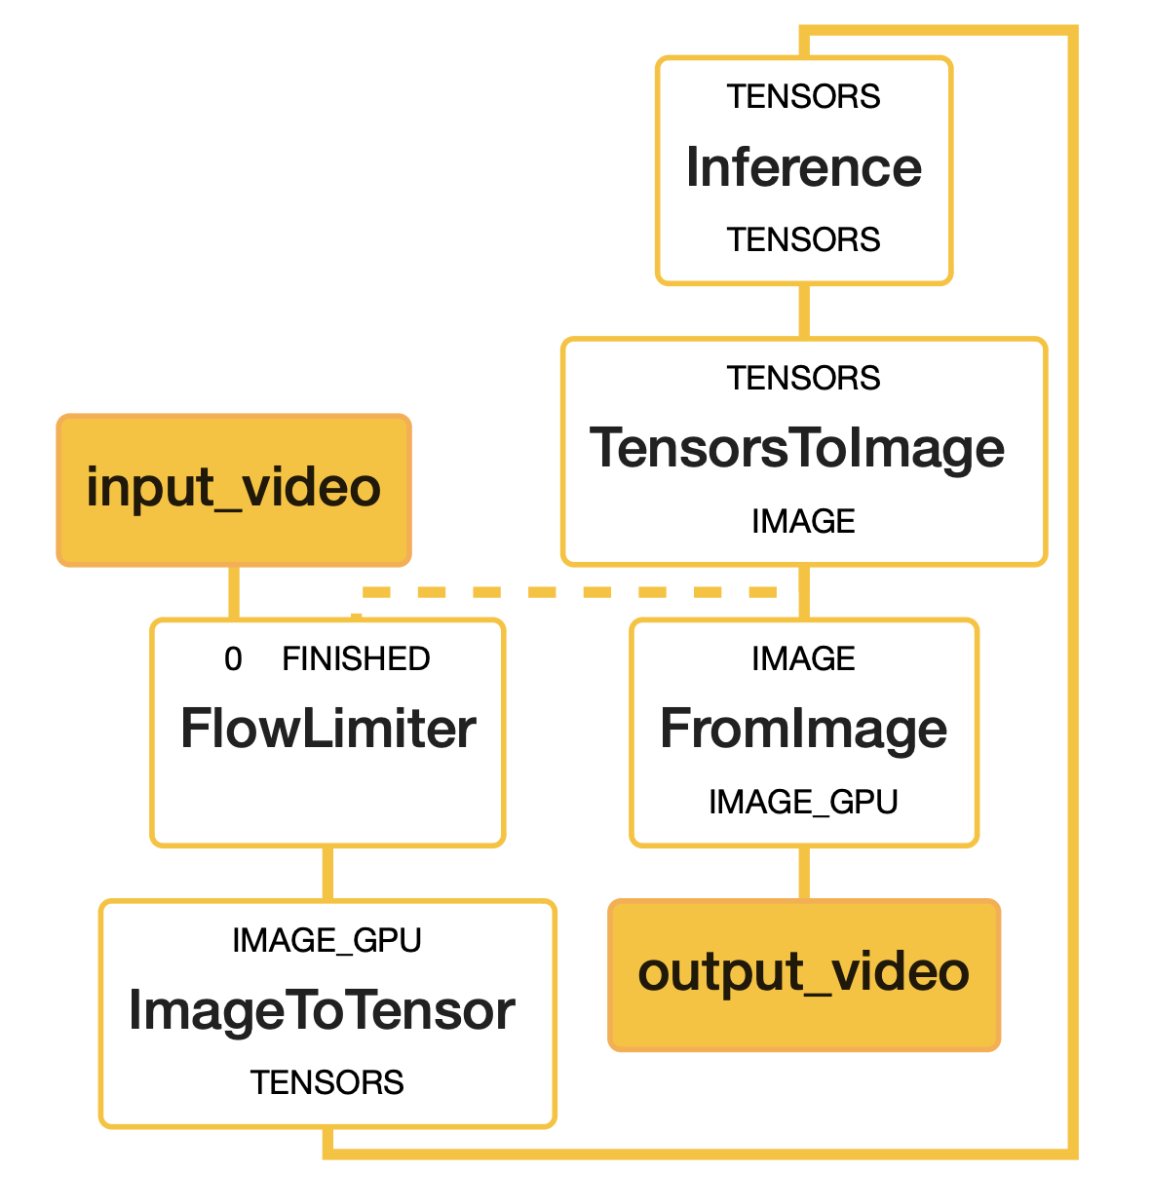
\includegraphics[width=\linewidth]{images-mediapipe/pipline.png}
                        \label{ris:mediapipe}
                        \caption{Конвейер для инференса на MediaPipe}
                    \end{minipage}
                \end{center}
            \end{figure}

        \section{Обзор фреймворка TensorFlow Lite с GPU делегатом}
        TensorFlow Lite (TFLite) представляет собой облегчённую версию TensorFlow, специально разработанную для выполнения нейросетевых моделей на устройствах с ограниченными ресурсами, таких как смартфоны, планшеты и устройства с встраиваемыми процессорами. В отличие от полноценного TensorFlow, TFLite предлагает минимальную зависимость от внешних библиотек, малый размер бинарного файла и высокоэффективную работу на мобильных чипах. Одной из ключевых особенностей TFLite является возможность делегации инференса на ускорители: GPU, DSP, TPU. В рамках поставленной задачи основное внимание уделяется GPU-делегату, предназначенному для выполнения операций на графических процессорах, особенно актуальному в задачах real-time обработки, таких как AR и компьютерное зрение.
        
            \subsection{Архитектура TFLite}
            TensorFlow Lite состоит из следующих основных компонентов:
            \begin{itemize}
                \item[-] Converter — инструмент для преобразования модели TensorFlow в оптимизированный формат FlatBuffer (.tflite), включая возможность квантования.
                \item[-] Interpreter — основной исполнитель модели, поддерживающий плагины-делегаты (delegates) и позволяющий выполнять модель на различных бэкендах.
                \item[-] Delegate — расширение, передающее выполнение определённых операций на специализированные ускорители.
                \item[-] Kernel Registry — таблица с реализациями всех поддерживаемых операций и их соответствием каждому типу делегата.
            \end{itemize}
        
            \subsection{GPU Delegate: назначение и архитектура}
            GPU Delegate в TFLite используется для выполнения инференса нейросетевых моделей с использованием графических процессоров, поддерживающих OpenGL ES 3.1+ или Vulkan. Главная цель — минимизация латентности при сохранении энергоэффективности и оптимизации работы в мобильных средах. Делегат позволяет параллельно обрабатывать тензоры с высокой пропускной способностью, особенно эффективен для свёрточных слоёв и операций типа element-wise.
            
            TFLite GPU Delegate реализован как плагин к интерпретатору. Он перехватывает граф операций при инициализации интерпретатора и заменяет стандартные реализации на GPU-ориентированные.
        
            Процесс делегации включает несколько этапов:
            \begin{enumerate}
                \item \textbf{Определение поддерживаемых операторов} — при инициализации интерпретатор вызывает GPU Delegate, который проверяет граф модели и определяет, какие из операций могут быть выполнены на GPU.
                \item \textbf{Переопределение подграфов} — соответствующие подграфы выделяются и переводятся в представление, пригодное для выполнения на GPU.
                \item \textbf{Компиляция шейдеров} — для каждой операции создаются OpenGL/Vulkan-шейдеры. Эти шейдеры компилируются на устройстве либо при запуске, либо заранее.
                \item \textbf{Выполнение модели} — на этапе инференса интерпретатор направляет входные тензоры на GPU, выполняется вычисление, и результаты возвращаются на CPU (при необходимости).
            \end{enumerate}
        
            \begin{figure}[h]
                \centering
                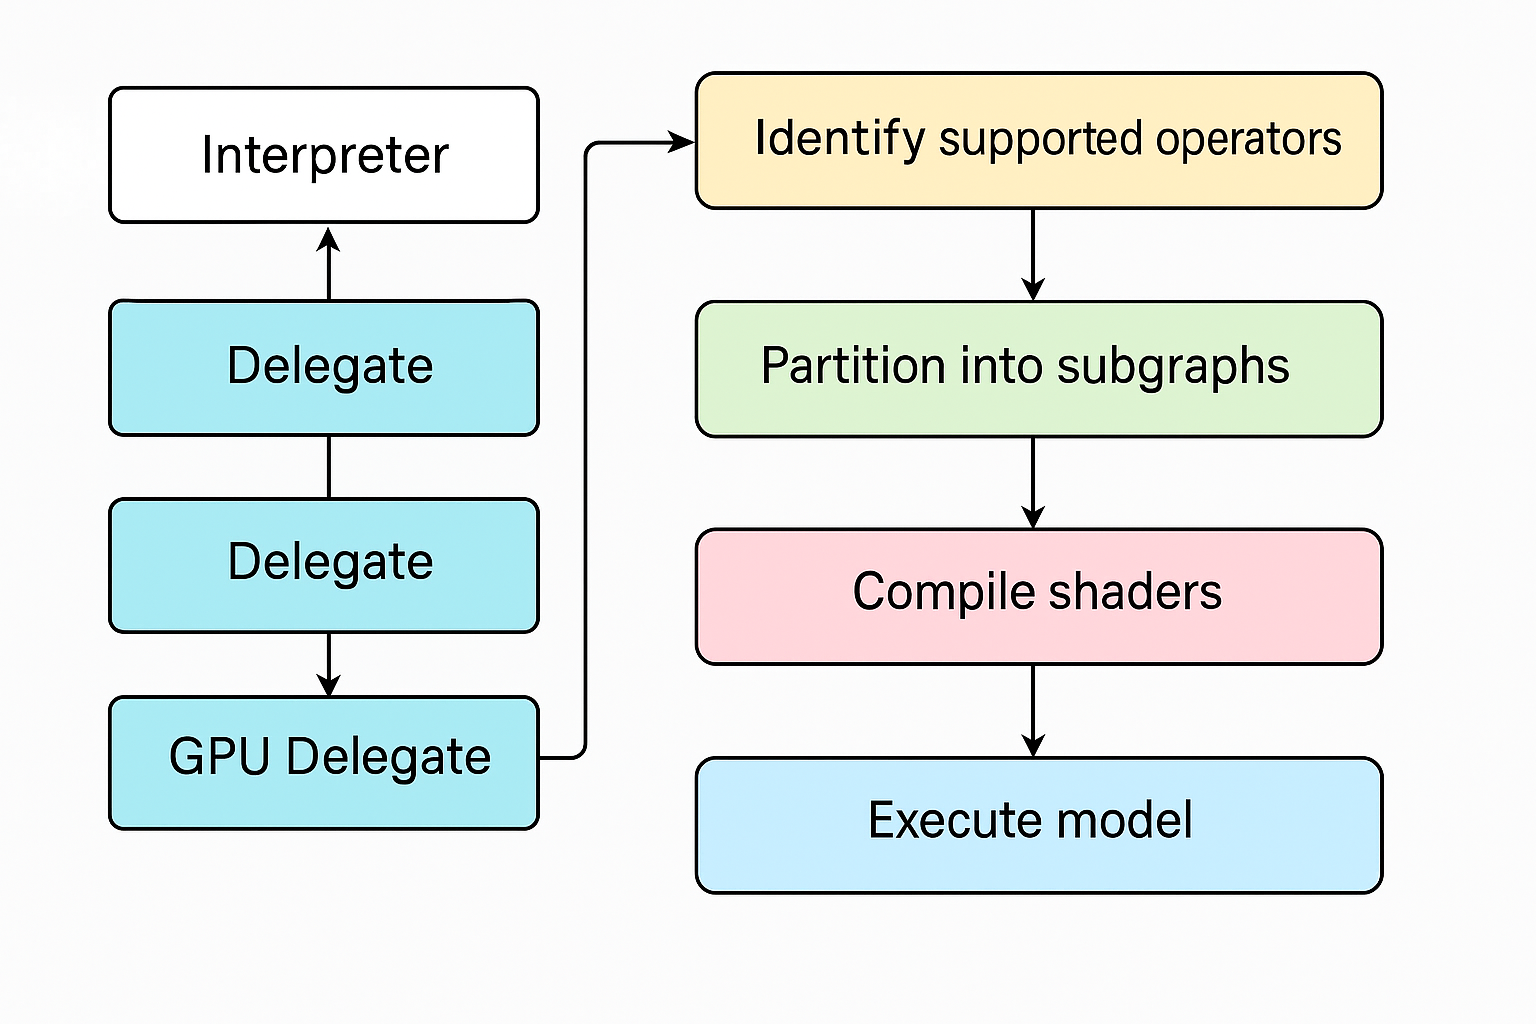
\includegraphics[width=0.6\linewidth]{images-tflite/arch.png}
                \caption{Схема делегации операций на GPU в TFLite}
                \label{ris:tflite_gpu_delegate}
                \vspace*{20pt}
            \end{figure}
            
            Поддерживаются как 16-битные (float16), так и 32-битные (float32) типы. Использование float16 даёт преимущества в скорости и потреблении памяти, особенно на устройствах с поддержкой half-precision операций.
        
            Несмотря на преимущества, делегат имеет ряд ограничений. Во-первых, не все операторы TFLite поддерживаются GPU Delegate. Также могут присутствовать высокие накладные расходы на запуск для малых моделей и ограниченная поддержка квантизованных моделей. Устройство может не поддерживать OpenGL ES 3.1+ или Vulkan, и компиляция шейдеров может занимать значительное время (особенно при первом запуске).

        \section{Тестирование пайплайна}
            \subsection{Оценка времени выполнения (Latency)}
            Тестирование охватывало два устройства, существенно отличающихся по архитектуре и вычислительным возможностям: мобильный смартфон Huawei P20 Pro на базе графического процессора ARM Mali-G72 MP12, а также ноутбук с дискретной графикой AMD Radeon Pro 5700 XT. Такой выбор устройств позволяет сопоставить производительность мобильных и десктопных GPU в задаче высокопроизводительного real-time инференса.
            
            Перед непосредственным измерением времени выполнения производился прогрев модели: первые 10 итераций инференса исключались из финальной оценки, что обеспечивало стабилизацию частоты графического процессора и избегало влияния начального старта. Далее, для каждой из реализаций — шейдерная реализация с использованием фрагментного шейдера, MediaPipe и TFLite GPU delegate — проводилось 50 запусков модели ESPCN (без учёта стартовых 10), на основе которых вычислялось среднее время одного инференса.

            \begin{figure}[h]
                \vspace*{-15pt}
                \centering
                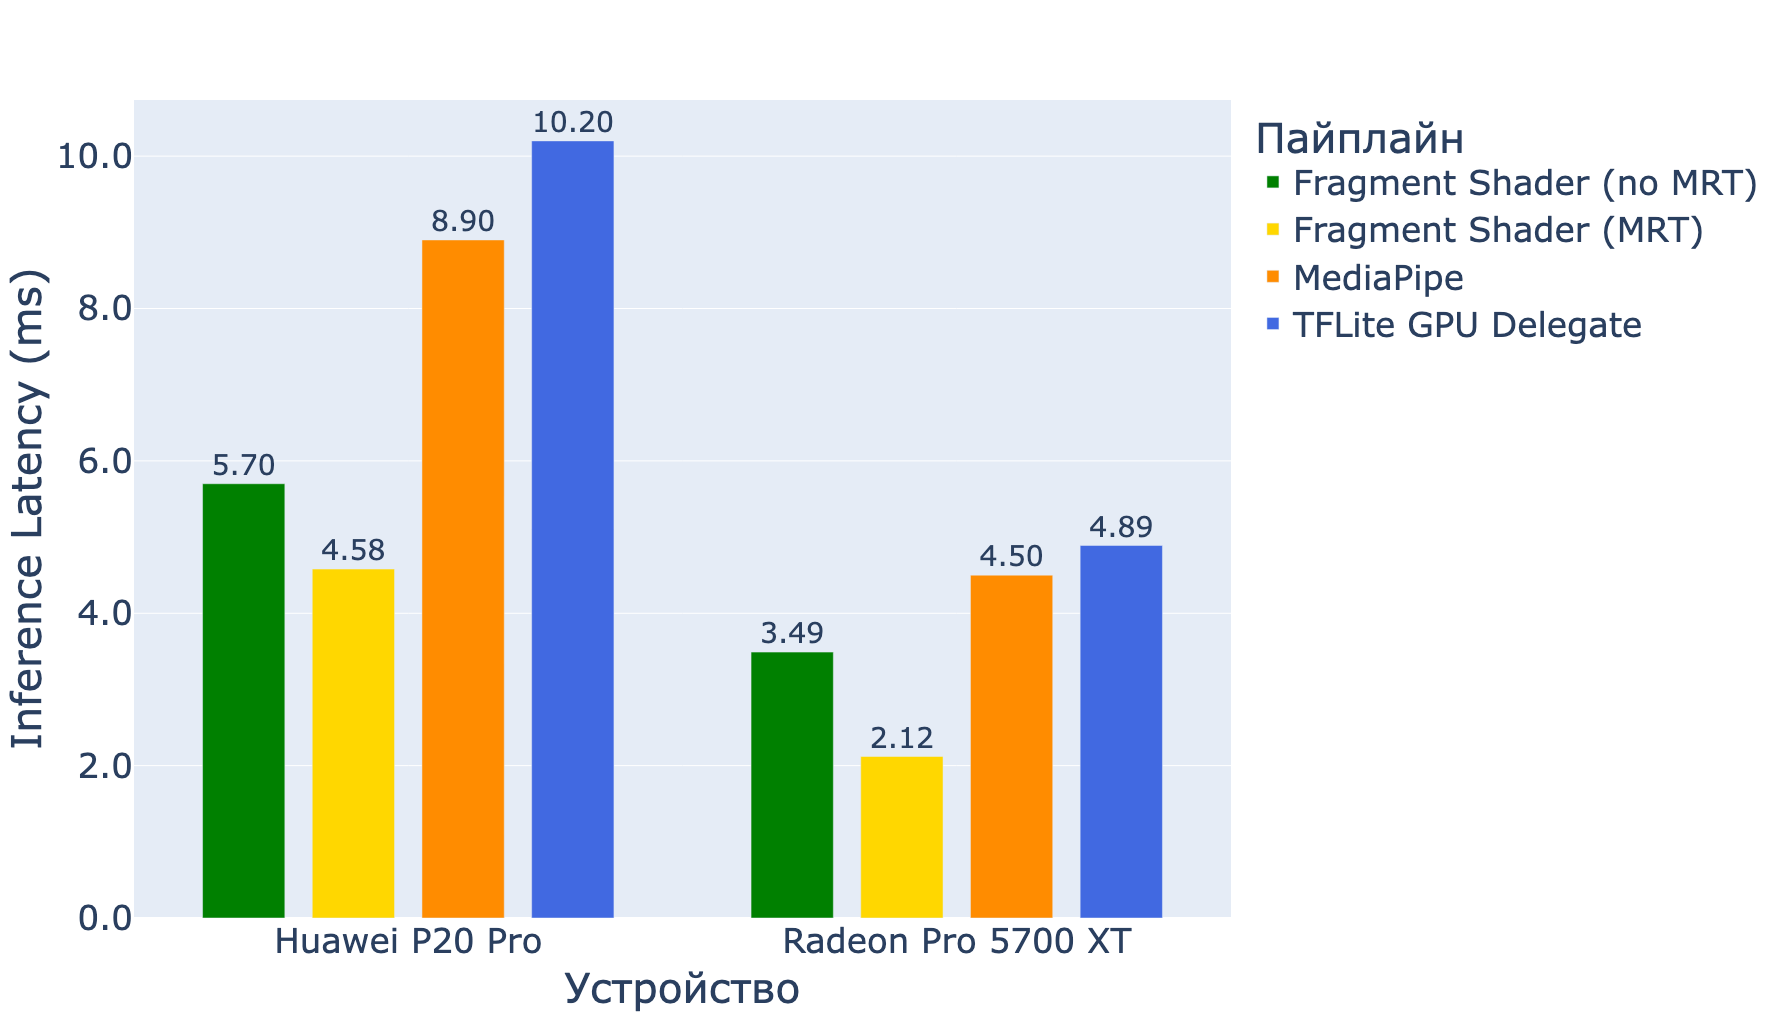
\includegraphics[width=0.98\linewidth]{images-tests/graphic.png}
                \caption{Сравнение латентности инференса модели ESPCN на различных GPU и пайплайнах}
                \label{ris:graphic}
                \vspace*{20pt}
            \end{figure}
            
            Следует отметить, что в реализованном пайплайне были применены две различные стратегии шейдерной компоновки: использование фрагментных шейдеров с MRT (Multiple Render Targets) и без него. Выбор между ними определялся профилированием на каждой платформе с целью достижения минимальной латентности. Для Huawei P20 Pro наиболее эффективной оказалась реализация на фрагментных шейдерах с MRT, как и для Radeon Pro 5700 XT.
            
            Как видно, шейдерная реализация (в обоих режимах) демонстрирует значительное преимущество по времени исполнения над MediaPipe и TFLite. Так, на Huawei P20 Pro пайплайн на фрагментных шейдерах обеспечил среднюю латентность 5.3 мс, тогда как MediaPipe — 8.9 мс, а TFLite — 10.2 мс. Разница ещё более выражена на десктопной системе: шейдерная реализация обеспечивает латентность в пределах 2.1–3.5 мс, тогда как у MediaPipe и TFLite — свыше 4 мс.
            
            Полученные результаты демонстрируют, что при грамотной организации вычислительного графа модели и правильном выборе GPU-ориентированных примитивов реализованный пайплайн способен значительно опережать существующие решения, при этом не требуя сторонних библиотек или платформенных зависимостей. Особенно ощутимо преимущество в условиях мобильного инференса, где время отклика критически важно для обеспечения качества пользовательского опыта в задачах дополненной реальности и компьютерного зрения в реальном времени.
            
            Кроме того, стоит отметить, что при использовании фрагментных шейдеров отсутствуют накладные расходы на управление глобальными вычислительными блоками (workgroup), что особенно актуально для моделей типа ESPCN, где объём вычислений внутри одного слоя относительно невелик, но требует высокой плотности пиксельных операций. Использование MRT также позволило сократить число рендер-проходов, минимизируя накладные расходы, связанные с переключением буферов и повторной компиляцией шейдеров.

            \subsection{Временные издержки на передачу данных между GPU и CPU}
            Одним из важных аспектов построения эффективного инференс-конвейера является минимизация количества пересылок данных между памятью GPU и CPU. Такие операции зачастую сопряжены с высокой латентностью и могут стать причиной значительных потерь в случае неэффективной архитектуры. В данной работе была проведена серия экспериментов, направленных на количественную оценку времени, затрачиваемого на передачу изображений между видеопамятью и оперативной памятью устройства, с использованием стандартных API: glReadPixels() и glTexSubImage2D().

            В качестве тестового набора были выбраны изображения с разрешением 720p и 1080p в формате RGBA32F. Для каждой из операций (GPU → CPU и CPU → GPU) выполнялось по 100 повторений на одном и том же наборе из 10 изображений. Все измерения проводились в режиме повышенной производительности устройств, с предварительной инициализацией текстур и фреймбуферов, чтобы исключить влияние на результаты времени выделения ресурсов.
            
            \begin{table}[h!]
                \centering
                \caption{Время передачи данных между GPU и CPU для различных устройств и разрешений}
                \vspace*{10pt}
                \begin{tabular}{|l|c|c|c|}
                    \hline
                    Устройство & Разрешение & GPU → CPU (мс) & CPU → GPU (мс) \\
                    \hline
                    Huawei P20 Pro     & 720p  & 5.02 & 3.71 \\
                                       & 1080p & 8.16 & 5.53 \\
                    \hline
                    Radeon Pro 5700 XT & 720p  & 3.11 & 2.58 \\
                                       & 1080p & 5.79 & 4.12 \\
                    \hline
                \end{tabular}
            \end{table}

            Результаты явно демонстрируют, что стоимость передачи данных между GPU и CPU пропорциональна разрешению изображений и составляет до 8.2 мс на мобильных устройствах и до 5.8 мс на десктопных. Эти значения весьма существенны при целевой частоте обновления кадров выше 30 FPS. В этой связи преимуществом предложенного пайплайна является полное отсутствие необходимости передачи промежуточных данных на CPU: весь инференс выполняется строго внутри графического конвейера, в текстурах и буферах кадра.

            Такой подход не только снижает задержки, но и уменьшает общую нагрузку на системную память, обеспечивая более предсказуемое поведение и лучшую масштабируемость, особенно в условиях одновременной работы нескольких графических задач.

            \subsection{Затраты на инициализацию пайплайна}
            Ещё одним важным параметром, влияющим на общую отзывчивость системы и пригодность реализованного пайплайна к использованию в real-time сценариях, является время инициализации и объём занимаемой памяти. Было произведено измерение времени запуска самого пайплайна инференса (без загрузки модели) и времени загрузки модели ESPCN отдельно. Все замеры проводились на десктопной системе с GPU Radeon Pro 5700 XT.
            
            \begin{table}[h!]
                \centering
                \caption{Время и количество задействованной памяти для инициализации пайплайна и загрузки модели}
                \vspace*{10pt}
                \begin{tabular}{|l|l|}
                    \hline
                    Параметр & Значение \\
                    \hline
                    Время инициализации пайплайна  & 47 мс \\
                    Объём памяти при инициализации & 42.3 МБ \\
                    Время загрузки модели ESPCN    & 29 мс \\
                    Объём памяти модели ESPCN      & 101.4 МБ \\
                    \hline
                \end{tabular}
            \end{table}

            Таким образом, общий запуск системы (инициализация + загрузка модели) укладывается в $\sim 76$ мс, что делает возможным её применение в интерактивных приложениях, не требующих предварительной предзагрузки. Низкие накладные расходы также означают, что пайплайн может использоваться динамически, например, в сценариях, где модель запускается и выгружается в зависимости от пользовательского действия.

            Низкое потребление памяти делает реализацию применимой даже на устройствах с ограниченными ресурсами, включая бюджетные мобильные платформы. Временные и пространственные характеристики пайплайна масштабируются линейно с ростом числа параметров модели, что делает архитектуру предсказуемой и контролируемой при добавлении новых моделей или расширении существующей.

            В данной главе содержатся основные полученные результаты дипломной работы. В начале был произведён краткий обзор фреймворков MediaPipe, TFLite и основных элементов их конвейеров. Приведён конвейер для фреймворка MediaPipe, с которым будет сравниваться реализованный пайплайн. Формализованы критерии эффективности использования нейросетей на GPU и описаны критерии для тестирования построенного пайплайна. Произведены замеры времени выполнения, задержки при передаче CPU->GPU и инициализации для реализованного пайплайна, MediaPipe и TFLite с GPU delegate. Проанализированы полученные результаты.
            
    \chapter*{ЗАКЛЮЧЕНИЕ}
    \addcontentsline{toc}{chapter}{ЗАКЛЮЧЕНИЕ}
    В ходе дипломной работы:
    \begin{enumerate}
        \item Произведен анализ существующих реализаций GPU пайплайнов и их особенностей. Показано, что главном проблемой является отсутствие фреймворков с поддержкой аппаратных структур данных GPU для входа: нельзя без потерь по времени передать выход модели напрямую в рендер пайплайн. Происходит через конвертацию GPU->CPU->GPU, что является медленной операций.
        \item Выбрана модель для построения конвейера. Ею стала ESPCN из-за довольно прозрачной архитектуры (три слоя Conv2D, слой Subpixel и слой activation).
        \item Сконструирована общая архитектура пайплайна. Она состоит из 4 основных этапов: преобразование модели в удобный для работы формат, загрузка модели и манипуляции с ней, генерация вычислительного графа и необходимая предобработка, выполнение соответствующих операторов для обработки модели.
        \item Согласно разработанной архитектуре, был реализован пайплайн на языке программирования С++, в основе которого лежит движок OpenGL.
        \item Написан скрипт для конвертации модели из формата .h5 (формат в котором хранится модель, обученная фреймворком TensorFlow) в json файл.
        \item Разработана архитектура обработки данных на шейдерах (структура вершинного и фрагментного шейдера). Также написаны шаблоны фрагментных шейдеров для слоев Conv2D, Activation и Subpixel.
        \item Проанализированы результаты сравнения построенного пайплайна с фреймворками MediaPipe и TFLite с GPU delegate.
    \end{enumerate}

    Задача эффективного использования нейронных сетей на графических процессорах и её применение является довольно сложной темой. В данной работе был реализован GPU-only пайплайн для инференса модели ESPCN с использованием фрагментных шейдеров на мобильных GPU. В итоге реализованный пайплайн показывает хорошие результаты инференса на модели ESPCN, имея латентность в районе $2.12-5.7$ мс, в зависимости от устройства и режима использования, в то время как лидирующие в этой сфере фреймворки — MediaPipe и TFLite с GPU delegate — показали в тех же условиях латентность в диапазоне от 4.5 до 10.2 мс.

    \chapter*{\large СПИСОК ИСПОЛЬЗОВАННЫХ ИСТОЧНИКОВ}
    \addcontentsline{toc}{chapter}{СПИСОК ИСПОЛЬЗОВАННЫХ ИСТОЧНИКОВ}
    \hypertarget{sources}{}
    \begin{enumerate}
        \item \hypertarget{[1]}{}Google AI Edge. (2025). Introducing LiteRT: Google's high-performance runtime for on-device AI, formerly known as TensorFlow Lite [Электронный ресурс]. Google AI Edge. – Режим доступа: \href{https://ai.google.dev/edge/litert}{https://ai.google.dev/edge/litert}. – Дата доступа: 16.05.2025.
        
        \item \hypertarget{[2]}{}PyTorch Foundation. (2025). PyTorch Mobile: End-to-end workflow from Training to Deployment for iOS and Android mobile devices [Электронный ресурс]. PyTorch. – Режим доступа: \href{https://pytorch.org/mobile/home/}{https://pytorch.org/mobile/home/}. – Дата доступа: 16.05.2025.
        
        \item \hypertarget{[3]}{}Apple Inc. (н.д.). Core ML | Apple Developer Documentation [Электронный ресурс]. Apple Inc. – Н/Д: Apple Inc. – Режим доступа: \href{https://developer.apple.com/documentation/coreml/}{https://developer.apple.com/documentation/coreml/}. – Дата доступа: 16.05.2025.
        
        \item \hypertarget{[4]}{}Xiaotang Jiang (2020). MNN: A Universal and Efficient Inference Engine / Xiaotang Jiang, Huan Wang, Yiliu Chen, Ziqi Wu, Lichuan Wang, Bin Zou, Yafeng Yang, Zongyang Cui, Yu Cai, Tianhang Yu, Chengfei Lv, Zhihua Wu. [Электронный ресурс]: Proceedings of the 3rd MLSys Conference. – Austin, TX, USA, 2020. – Режим доступа: \href{https://arxiv.org/pdf/2002.12418}{https://arxiv.org/pdf/2002.12418}. – Дата доступа: 16.05.2025.

        \item \hypertarget{[5]}{}NCNN Foundation. – Austin, TX, USA, 2020. – Режим доступа: \href{https://github.com/Tencent/ncnn}{https://github.com/Tencent/ncnn}. – Дата доступа: 16.05.2025.

        \item \hypertarget{[6]}{} TNN Foundation. – Режим доступа: \href{https://github.com/Tencent/TNN}{https://github.com/Tencent/TNN}. – Дата доступа: 16.05.2025.

        \item \hypertarget{[7]}{} Bolt AI. Huawei Noah. – Режим доступа: \href{https://zhuanlan.zhihu.com/p/317111024}{https://zhuanlan.zhihu.com/p/317111024}. – Дата доступа: 16.05.2025.

        \item \hypertarget{[8]}{} Mace AI. Xiami. – Режим доступа: \href{https://github.com/XiaoMi/mace}{https://github.com/XiaoMi/mace}. – Дата доступа: 16.05.2025.

        \item \hypertarget{[9]}{} Anakin AI. PaddlePaddle. – Режим доступа: \href{https://github.com/PaddlePaddle/Anakin}{https://github.com/PaddlePaddle/Anakin}. – Дата доступа: 16.05.2025.
        
        \item \hypertarget{[10]}{}Shi W. et al. Real-time single image and video super-resolution using an efficient sub-pixel convolutional neural network //Proceedings of the IEEE conference on computer vision and pattern recognition. – 2016. – С. 1874-1883. [Электронный ресурс]: Twitter, Inc. – Режим доступа: \href{https://www.cv-foundation.org/openaccess/content_cvpr_2016/papers/Shi_Real-Time_Single_Image_CVPR_2016_paper.pdf}{https://www.cv-foundation.org/openaccess/content\_cvpr\_2016/papers/Shi\_Real-Time\_Single\_Image\_CVPR\_2016\_paper.pdf}. – Дата доступа: 16.05.2025.

        \item \hypertarget{[11]}{} Netron App. – Режим доступа: \href{https://netron.app}{https://netron.app}. – Дата доступа: 16.05.2025.
        
        \item \hypertarget{[12]}{}Lugaresi C. et al. Mediapipe: A framework for building perception pipelines / Lugaresi C., Tang J., Nash H., McClanahan C., Uboweja E., Hays M., Zhang F., Chang C.-L., Yong M.G., Lee J. – Режим доступа: \href{https://arxiv.org/abs/1906.08172}{https://arxiv.org/abs/1906.08172}. – Дата доступа: 16.05.2025.
        
        \item \hypertarget{[13]}{} Image 1.1. Архитектура пайплайн с использованием
        сторонних фреймворков – Режим доступа: \href{https://ars.els-cdn.com/content/image/1-s2.0-S0925231224013997-gr3.jpg}{https://ars.els-cdn.com/content/image/1-s2.0-S0925231224013997-gr3.jpg}. – Дата доступа: 16.05.2025.
    \end{enumerate}
    
\end{document}
